% Options for packages loaded elsewhere
% Options for packages loaded elsewhere
\PassOptionsToPackage{unicode}{hyperref}
\PassOptionsToPackage{hyphens}{url}
\PassOptionsToPackage{dvipsnames,svgnames,x11names}{xcolor}
%
\documentclass[
  11pt]{article}
\usepackage{xcolor}
\usepackage{amsmath,amssymb}
\setcounter{secnumdepth}{5}
\usepackage{iftex}
\ifPDFTeX
  \usepackage[T1]{fontenc}
  \usepackage[utf8]{inputenc}
  \usepackage{textcomp} % provide euro and other symbols
\else % if luatex or xetex
  \usepackage{unicode-math} % this also loads fontspec
  \defaultfontfeatures{Scale=MatchLowercase}
  \defaultfontfeatures[\rmfamily]{Ligatures=TeX,Scale=1}
\fi
\usepackage{lmodern}
\ifPDFTeX\else
  % xetex/luatex font selection
\fi
% Use upquote if available, for straight quotes in verbatim environments
\IfFileExists{upquote.sty}{\usepackage{upquote}}{}
\IfFileExists{microtype.sty}{% use microtype if available
  \usepackage[]{microtype}
  \UseMicrotypeSet[protrusion]{basicmath} % disable protrusion for tt fonts
}{}
% Make \paragraph and \subparagraph free-standing
\makeatletter
\ifx\paragraph\undefined\else
  \let\oldparagraph\paragraph
  \renewcommand{\paragraph}{
    \@ifstar
      \xxxParagraphStar
      \xxxParagraphNoStar
  }
  \newcommand{\xxxParagraphStar}[1]{\oldparagraph*{#1}\mbox{}}
  \newcommand{\xxxParagraphNoStar}[1]{\oldparagraph{#1}\mbox{}}
\fi
\ifx\subparagraph\undefined\else
  \let\oldsubparagraph\subparagraph
  \renewcommand{\subparagraph}{
    \@ifstar
      \xxxSubParagraphStar
      \xxxSubParagraphNoStar
  }
  \newcommand{\xxxSubParagraphStar}[1]{\oldsubparagraph*{#1}\mbox{}}
  \newcommand{\xxxSubParagraphNoStar}[1]{\oldsubparagraph{#1}\mbox{}}
\fi
\makeatother


\usepackage{longtable,booktabs,array}
\usepackage{calc} % for calculating minipage widths
% Correct order of tables after \paragraph or \subparagraph
\usepackage{etoolbox}
\makeatletter
\patchcmd\longtable{\par}{\if@noskipsec\mbox{}\fi\par}{}{}
\makeatother
% Allow footnotes in longtable head/foot
\IfFileExists{footnotehyper.sty}{\usepackage{footnotehyper}}{\usepackage{footnote}}
\makesavenoteenv{longtable}
\usepackage{graphicx}
\makeatletter
\newsavebox\pandoc@box
\newcommand*\pandocbounded[1]{% scales image to fit in text height/width
  \sbox\pandoc@box{#1}%
  \Gscale@div\@tempa{\textheight}{\dimexpr\ht\pandoc@box+\dp\pandoc@box\relax}%
  \Gscale@div\@tempb{\linewidth}{\wd\pandoc@box}%
  \ifdim\@tempb\p@<\@tempa\p@\let\@tempa\@tempb\fi% select the smaller of both
  \ifdim\@tempa\p@<\p@\scalebox{\@tempa}{\usebox\pandoc@box}%
  \else\usebox{\pandoc@box}%
  \fi%
}
% Set default figure placement to htbp
\def\fps@figure{htbp}
\makeatother





\setlength{\emergencystretch}{3em} % prevent overfull lines

\providecommand{\tightlist}{%
  \setlength{\itemsep}{0pt}\setlength{\parskip}{0pt}}



 
\usepackage[]{natbib}
\bibliographystyle{econ}


\usepackage{graphicx}
\usepackage{bbm}
\usepackage{amssymb}
\usepackage{amsmath}
\usepackage[nomarginpar]{geometry}
\usepackage{setspace}
\usepackage{natbib}
\usepackage{lscape}
\usepackage{rotating}
\usepackage{tabularx, calc}
\usepackage{threeparttable}
\usepackage{picinpar}  
\usepackage{longtable}
\usepackage{ae}
\usepackage{float}
\usepackage{morefloats}
\usepackage{palatino}
\usepackage{hyperref}
\usepackage{color}
\usepackage{adjustbox}
\usepackage{booktabs} 
\usepackage{ulem}
\usepackage{ragged2e}
\usepackage{changepage}
\usepackage{longtable}
%\usepackage{graphics}
%\usepackage[tableposition=top]{caption}

\geometry{left=1.0in,right=1.0in,top=1.0in,bottom=1.0in}
\onehalfspacing
\makeatletter
\@ifpackageloaded{caption}{}{\usepackage{caption}}
\AtBeginDocument{%
\ifdefined\contentsname
  \renewcommand*\contentsname{Table of contents}
\else
  \newcommand\contentsname{Table of contents}
\fi
\ifdefined\listfigurename
  \renewcommand*\listfigurename{List of Figures}
\else
  \newcommand\listfigurename{List of Figures}
\fi
\ifdefined\listtablename
  \renewcommand*\listtablename{List of Tables}
\else
  \newcommand\listtablename{List of Tables}
\fi
\ifdefined\figurename
  \renewcommand*\figurename{Figure}
\else
  \newcommand\figurename{Figure}
\fi
\ifdefined\tablename
  \renewcommand*\tablename{Table}
\else
  \newcommand\tablename{Table}
\fi
}
\@ifpackageloaded{float}{}{\usepackage{float}}
\floatstyle{ruled}
\@ifundefined{c@chapter}{\newfloat{codelisting}{h}{lop}}{\newfloat{codelisting}{h}{lop}[chapter]}
\floatname{codelisting}{Listing}
\newcommand*\listoflistings{\listof{codelisting}{List of Listings}}
\makeatother
\makeatletter
\makeatother
\makeatletter
\@ifpackageloaded{caption}{}{\usepackage{caption}}
\@ifpackageloaded{subcaption}{}{\usepackage{subcaption}}
\makeatother
\usepackage{bookmark}
\IfFileExists{xurl.sty}{\usepackage{xurl}}{} % add URL line breaks if available
\urlstyle{same}
\hypersetup{
  pdftitle={Coding assignment (QSM class)},
  pdfauthor={Hyoungchul Kim},
  colorlinks=true,
  linkcolor={cyan},
  filecolor={Maroon},
  citecolor={cyan},
  urlcolor={cyan},
  pdfcreator={LaTeX via pandoc}}


\title{Coding assignment (QSM class)}
\author{Hyoungchul Kim}
\date{September 10, 2025}
\begin{document}
\def\spacingset#1{\renewcommand{\baselinestretch}%
{#1}\small\normalsize} \spacingset{1}


%%%%%%%%%%%%%%%%%%%%%%%%%%%%%%%%%%%%%%%%%%%%%%%%%%%%%%%%%%%%%%%%%%%%%%%%%%%%%%

\date{\href{https://github.com/hchulkim/qsm-class/blob/main/output/output.pdf}{Link to Latest version}\\ \vspace{1em}  Last updated September
10, 2025}
\title{Coding assignment (QSM class)\thanks{I acknowledge that I worked
with Coni, Yuxuan, and Eni. I also acknowledge that I used
\citet{chatgpt} and \citet{cursor} to help me with the coding. They were
mostly used for debugging and auto-completion. Thus, the main structure
of the code was all written by the author. All the codes were later
reviwed and finalized by the author.}}
\author{
Hyoungchul Kim\thanks{email: hchulkim@wharton.upenn.edu}\\
The Wharton School, University of Pennsylvania\\
}
\maketitle

\bigskip
\bigskip
\begin{abstract}
This is a coding assignment for the QSM class.
\end{abstract}

\bigskip

\newpage
\spacingset{1.2} % DON'T change the spacing!

\section{Use of programming
language}\label{sec-use-of-programming-language}

For questions 1-7, I used \texttt{R} programming language. I also used
\texttt{R} for most of the data cleaning and manipulation. For other
questions that requires more computationally intensive analyses
(modeling, etc.), I used \texttt{julia} programming language.

\section{Main data information}\label{sec-main-data-info}

I am using the 2022 LODES data from LEHD for my analysis. I obtained the
raw data for Philadelphia county from the LEHD website and aggregated
the data into tract-tract level. The process of cleaning the raw data
was conducted using the source code:
\texttt{src/R/01\_clean\_raw\_data.R}.

My primary analysis zone will be bilateral commuting flow within
Philadelphia county for the year 2022. This means I will not be
considering the flow where either the origin or the destination is
outside of Philadelphia county.

\subsection*{Q1}\label{q1}
\addcontentsline{toc}{subsection}{Q1}

As I mentioned in Section~\ref{sec-main-data-info}, I obtained bilateral
commuting flow data from LEHD LODES for the year 2022. I also downloaded
supporting data on the locations of the tracts or blocks underlying the
data. I downloaded them in the \texttt{input} folder. You can also use
\texttt{make\ raw} command to automatically download the raw
data.\footnote{Note that if you want to re-download the raw data, you
  must first use \texttt{make\ clean\_raw} command to remove the raw
  data in the \texttt{input} folder. Also note that if the original data
  was updated during the course of the semester, there is a likelihood
  that the new downloaded data might have different data structure that
  could affect the analysis.}

\subsection*{Q2}\label{q2}
\addcontentsline{toc}{subsection}{Q2}

For distance, I will use the distance between the centroids of the
origin and destination tracts. For this, I used \texttt{sf} package and
\texttt{tigris} package in R to calculate the distance between the
centroids of the origin and destination tracts. The source code is
available in \texttt{src/R/02\_calculate\_distance.R}. I also retained
the fixed effects estimates in the Appendix.

\subsection*{Q3}\label{q3}
\addcontentsline{toc}{subsection}{Q3}

I estimated the following linear model:

\[
\log(N_{ij}) = \theta_{i} + \lambda_{j} - \epsilon \kappa d_{ij} + e_{ij}\label{eq:distance}
\]

The estimation results are reported in the following table:

\clearpage

\begin{table}[!ht]
\centering
\caption{Estimation results}
\label{tab:est_results}

\begin{tabular}{l c}
\hline
 & Log of commuting flow \\
\hline
distance\_km          & $-0.07^{***}$ \\
                      & $(0.00)$      \\
\hline
Num. obs.             & $73326$       \\
Num. groups: w\_tract & $406$         \\
Num. groups: h\_tract & $408$         \\
R$^2$ (full model)    & $0.61$        \\
R$^2$ (proj model)    & $0.19$        \\
\hline
\multicolumn{2}{l}{\scriptsize{$^{***}p<0.001$; $^{**}p<0.01$; $^{*}p<0.05$}}
\end{tabular}

\end{table}

\footnotesize \textbf{Note}: This table presents estimation result of
the equation \ref{eq:distance}. \texttt{distance\_km} is the estimate of
the \(-\epsilon\kappa\). The value in the paranthesis is standard
error.\vspace{3em}

\normalsize

\section*{Q4}\label{q4}
\addcontentsline{toc}{section}{Q4}

After including all the \(ij\) pairs and adding in zero commuting flows,
I estimated the PPML model as follows:

\[
\log(\mathbb{E}[N_{ij}])= \theta_{i} + \lambda_{j} - \epsilon \kappa d_{ij} + e_{ij}\label{eq:ppml}
\]

The estimation results are reported in the following table (I also
retained the fixed effects estimates in the
\texttt{input/q4\_ppml\_fes.csv}):

\begin{table}[!ht]
\centering
\caption{Estimation results of the PPML model}
\label{tab:est_ppml}

\begin{tabular}{l c}
\hline
 & PPML \\
\hline
distance\_km          & $-0.12^{***}$ \\
                      & $(0.01)$      \\
\hline
Num. obs.             & $165648$      \\
Num. groups: w\_tract & $406$         \\
Num. groups: h\_tract & $408$         \\
Pseudo R$^2$          & $0.64$        \\
\hline
\multicolumn{2}{l}{\scriptsize{$^{***}p<0.001$; $^{**}p<0.01$; $^{*}p<0.05$}}
\end{tabular}

\end{table}

\footnotesize \textbf{Note}: This table presents estimation result of
the equation \ref{eq:ppml}. \texttt{distance\_km} is the estimate of the
\(-\epsilon\kappa\). The value in the paranthesis is standard
error.\vspace{3em}

\normalsize

We can clearly see that the estimate of the \(-\epsilon\kappa\) differs
from the estimate in the previous question. The absolute size of the
estimate is larger in the PPML model. Intuitively, I think this occurs
because the PPML model incorporates the zero commuting flows that were
neglected in the linear model. Since the zero commuting flows were not
fully incorporated in the linear model, the estimate in the linear model
was underestimating the effect of the travel-time cost on the commuting
flow. The estimate in the PPML model shifts downward to account for the
zero commuting flows.

Something to note is that in PPML, FEs are not always identified. In our
case, two FEs are not identified because there is no flow for any
tract-tract pair.

\section*{Q5}\label{q5}
\addcontentsline{toc}{section}{Q5}

\begin{enumerate}
\def\labelenumi{\arabic{enumi}.}
\tightlist
\item
  For \(ii\) pairs, we could add minimum distance from the centroid to
  the edge of the polygon geometry as the distance measure. While this
  is not a perfect measure, it still should work as a proxy for
  measuring the relative size of certain distance from traveling within
  the same tract. This also solves the zero distance issue. The only
  problem might be that this method could be bit ad-hoc and not
  consistent as we are just adding additional values only onto the
  \(ii\) pairs and not consider the \(ij\) pairs.
\end{enumerate}

Using this method, I get the following estimates for linear and PPML
models:

\begin{table}[!ht]
\centering
\caption{Estimation results of the linear model for $ii$ pairs}
\label{tab:est_linear_ii}

\begin{tabular}{l c}
\hline
 & Log of commuting flow \\
\hline
distance\_km          & $-0.07^{***}$ \\
                      & $(0.00)$      \\
\hline
Num. obs.             & $73326$       \\
Num. groups: w\_tract & $406$         \\
Num. groups: h\_tract & $408$         \\
R$^2$ (full model)    & $0.61$        \\
R$^2$ (proj model)    & $0.19$        \\
\hline
\multicolumn{2}{l}{\scriptsize{$^{***}p<0.001$; $^{**}p<0.01$; $^{*}p<0.05$}}
\end{tabular}

\end{table}

\begin{table}[!ht]
\centering
\caption{Estimation results of the PPML model for $ii$ pairs}
\label{tab:est_ppml_ii}

\begin{tabular}{l c}
\hline
 & PPML \\
\hline
distance\_km          & $-0.12^{***}$ \\
                      & $(0.01)$      \\
\hline
Num. obs.             & $165648$      \\
Num. groups: w\_tract & $406$         \\
Num. groups: h\_tract & $408$         \\
Pseudo R$^2$          & $0.64$        \\
\hline
\multicolumn{2}{l}{\scriptsize{$^{***}p<0.001$; $^{**}p<0.01$; $^{*}p<0.05$}}
\end{tabular}

\end{table}

\begin{enumerate}
\def\labelenumi{\arabic{enumi}.}
\setcounter{enumi}{1}
\tightlist
\item
  Another way would be to change the definition of the distance measure
  so that \(ii\) pairs will not have zero values. We leverage the fact
  that our data can become more granular. That is, we have information
  on the longitude and latitude of the centroid of the census block.
  After calculating the distance between two centroids of the census
  blocks, we can use mean of the all the block-level distances within
  the same tract-tract pair as the distance measure of the tract-tract
  pairs. This will give us non-zero distance for \(ii\) pairs.
\end{enumerate}

Using this method, I get the following estimates for linear and PPML
models:

\begin{table}[!ht]
\centering
\caption{Estimation results of the linear model for $ii$ pairs}
\label{tab:est_linear_ii_2}

\begin{tabular}{l c}
\hline
 & Log of commuting flow \\
\hline
distance\_km          & $-0.07^{***}$ \\
                      & $(0.00)$      \\
\hline
Num. obs.             & $73326$       \\
Num. groups: w\_tract & $406$         \\
Num. groups: h\_tract & $408$         \\
R$^2$ (full model)    & $0.61$        \\
R$^2$ (proj model)    & $0.19$        \\
\hline
\multicolumn{2}{l}{\scriptsize{$^{***}p<0.001$; $^{**}p<0.01$; $^{*}p<0.05$}}
\end{tabular}

\end{table}

\begin{table}[!ht]
\centering
\caption{Estimation results of the PPML model for $ii$ pairs}
\label{tab:est_ppml_ii_2}

\begin{tabular}{l c}
\hline
 & PPML \\
\hline
distance\_km          & $-0.12^{***}$ \\
                      & $(0.01)$      \\
\hline
Num. obs.             & $165648$      \\
Num. groups: w\_tract & $406$         \\
Num. groups: h\_tract & $408$         \\
Pseudo R$^2$          & $0.64$        \\
\hline
\multicolumn{2}{l}{\scriptsize{$^{***}p<0.001$; $^{**}p<0.01$; $^{*}p<0.05$}}
\end{tabular}

\end{table}

You can see that the estimates are very similar to the estimates in the
previous question. This suggests that perhaps the zero distance issue is
not a major issue in the analysis.

\section*{Q6}\label{q6}
\addcontentsline{toc}{section}{Q6}

\clearpage

\section*{Q7}\label{q7}
\addcontentsline{toc}{section}{Q7}

My code in \texttt{src/R/07\_create\_market\_access.R} creates the
market access variable. For each residential and workplace tract, I
calculate the market access variable using the definition in the
question. I posted the result in the Appendix. In the main document, I
will plot the map of the market access variable.

\begin{figure}

\begin{minipage}{0.50\linewidth}

\centering{

\pandocbounded{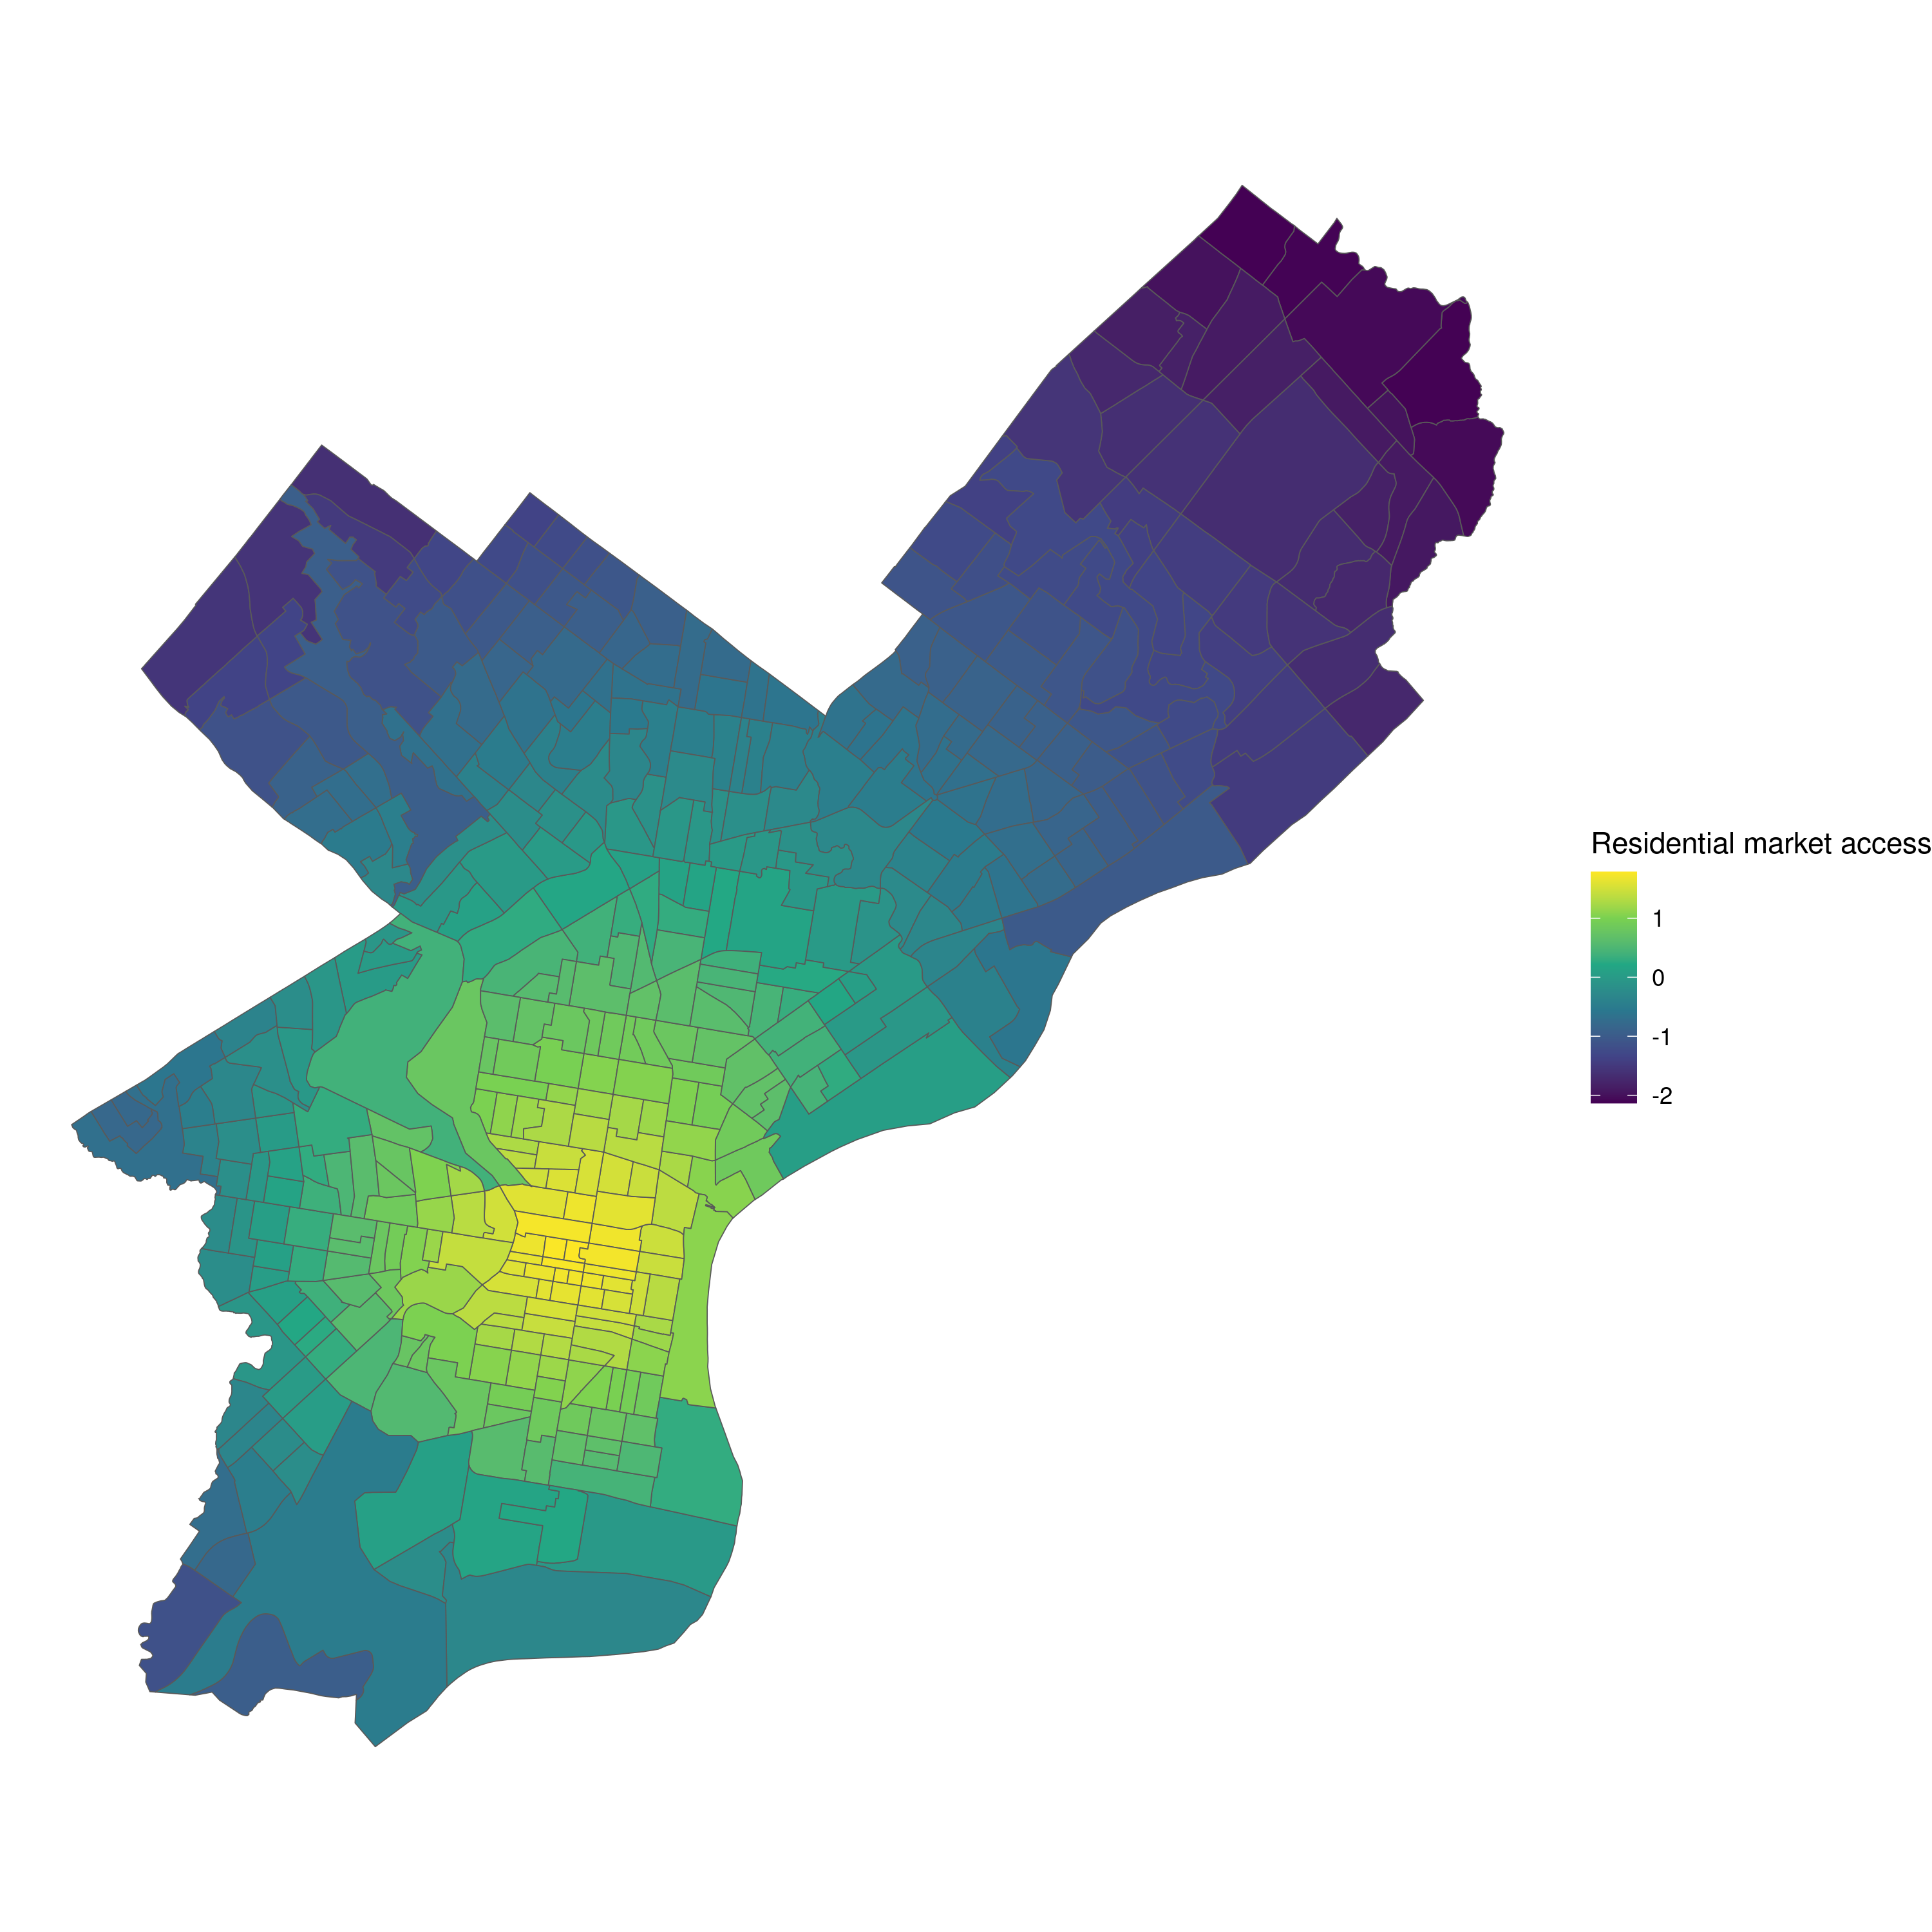
\includegraphics[keepaspectratio]{figures/residential_market_access.png}}

}

\subcaption{\label{fig-residential-market-access}Map of the residential
market access}

\end{minipage}%
%
\begin{minipage}{0.50\linewidth}

\centering{

\pandocbounded{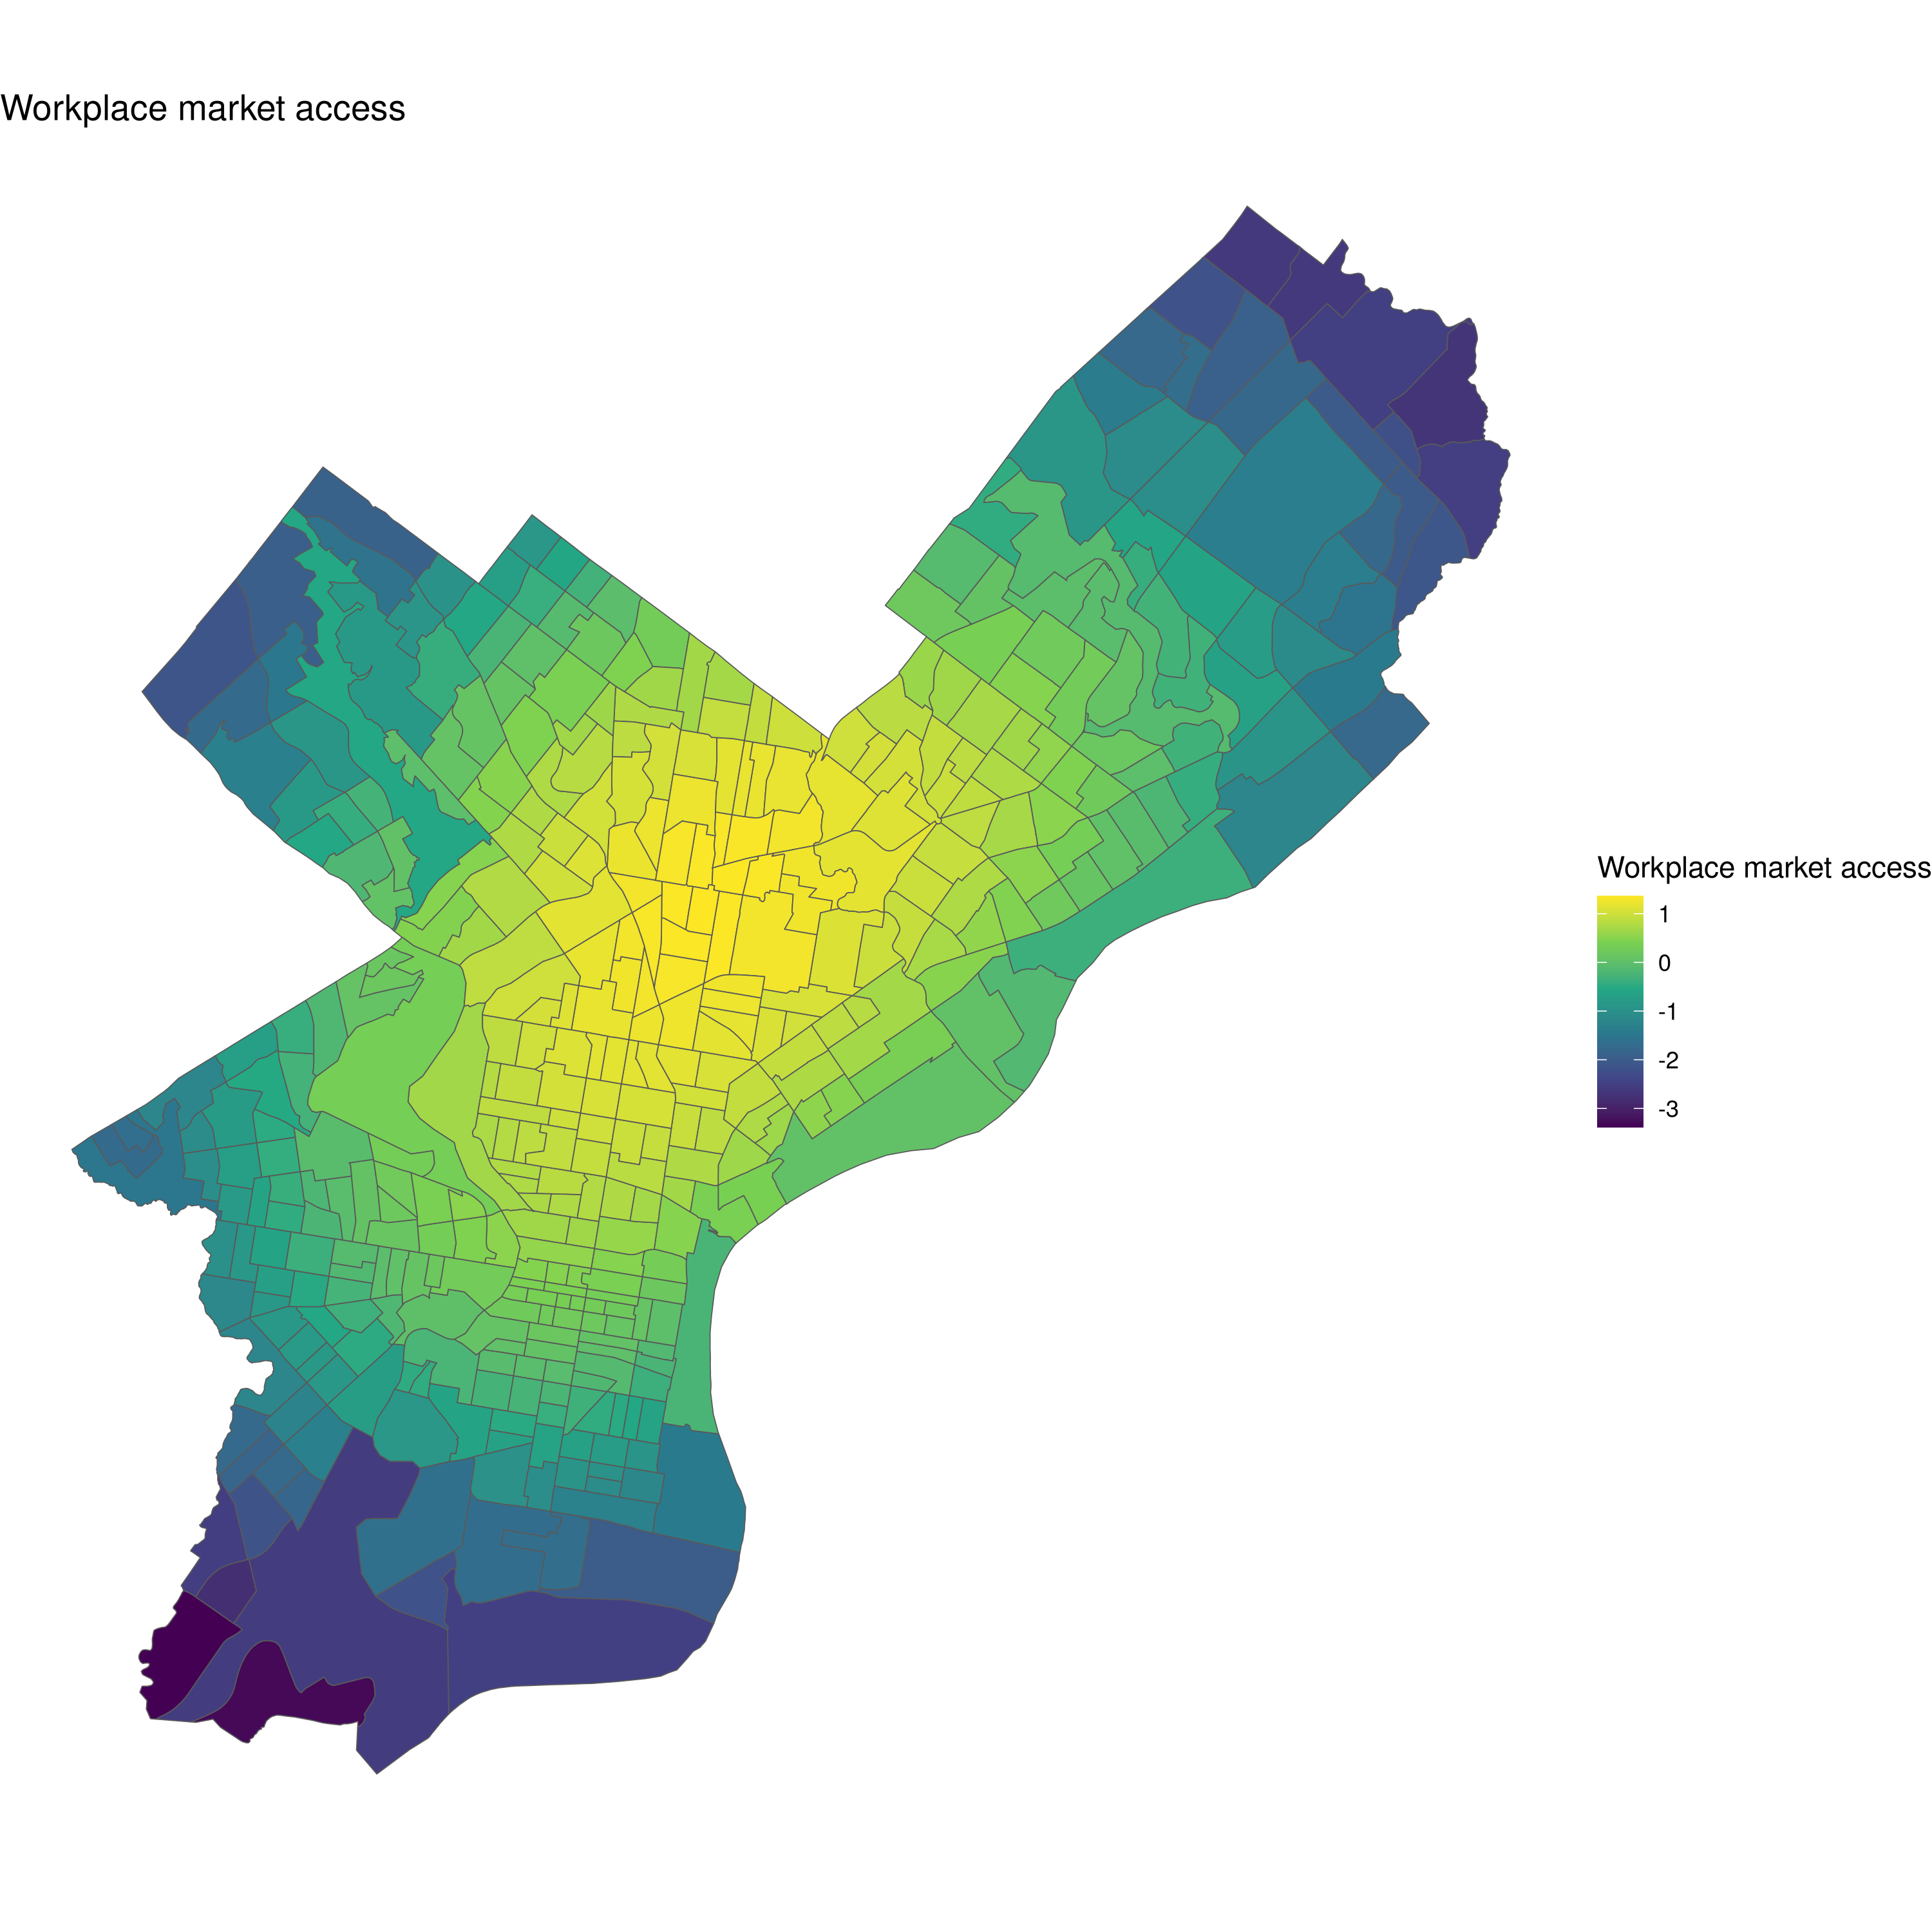
\includegraphics[keepaspectratio]{figures/workplace_market_access.png}}

}

\subcaption{\label{fig-workplace-market-access}Map of the workplace
market access}

\end{minipage}%

\end{figure}%

\footnotesize \textbf{Note}: This is the map (Philadelphia county) of
the market access variable. The color represents the market access
variable. The lighter the color, the higher the market access. The
values are normalized (z-score).

\normalsize

\clearpage

\section*{Q8}\label{q8}
\addcontentsline{toc}{section}{Q8}

I use two scripts to accomplish this. For data manipulation stage I use
\texttt{src/R/08\_fixed\_point\_algorithm.R} to create the sum of
bilateral commuting flow and the expotential terms. For implementing
fixed point algorithm, I use
\texttt{src/julia/08\_fixed\_point\_algorithm.jl}.

I plot the map of the market access again below:

\begin{figure}

\begin{minipage}{0.50\linewidth}

\centering{

\pandocbounded{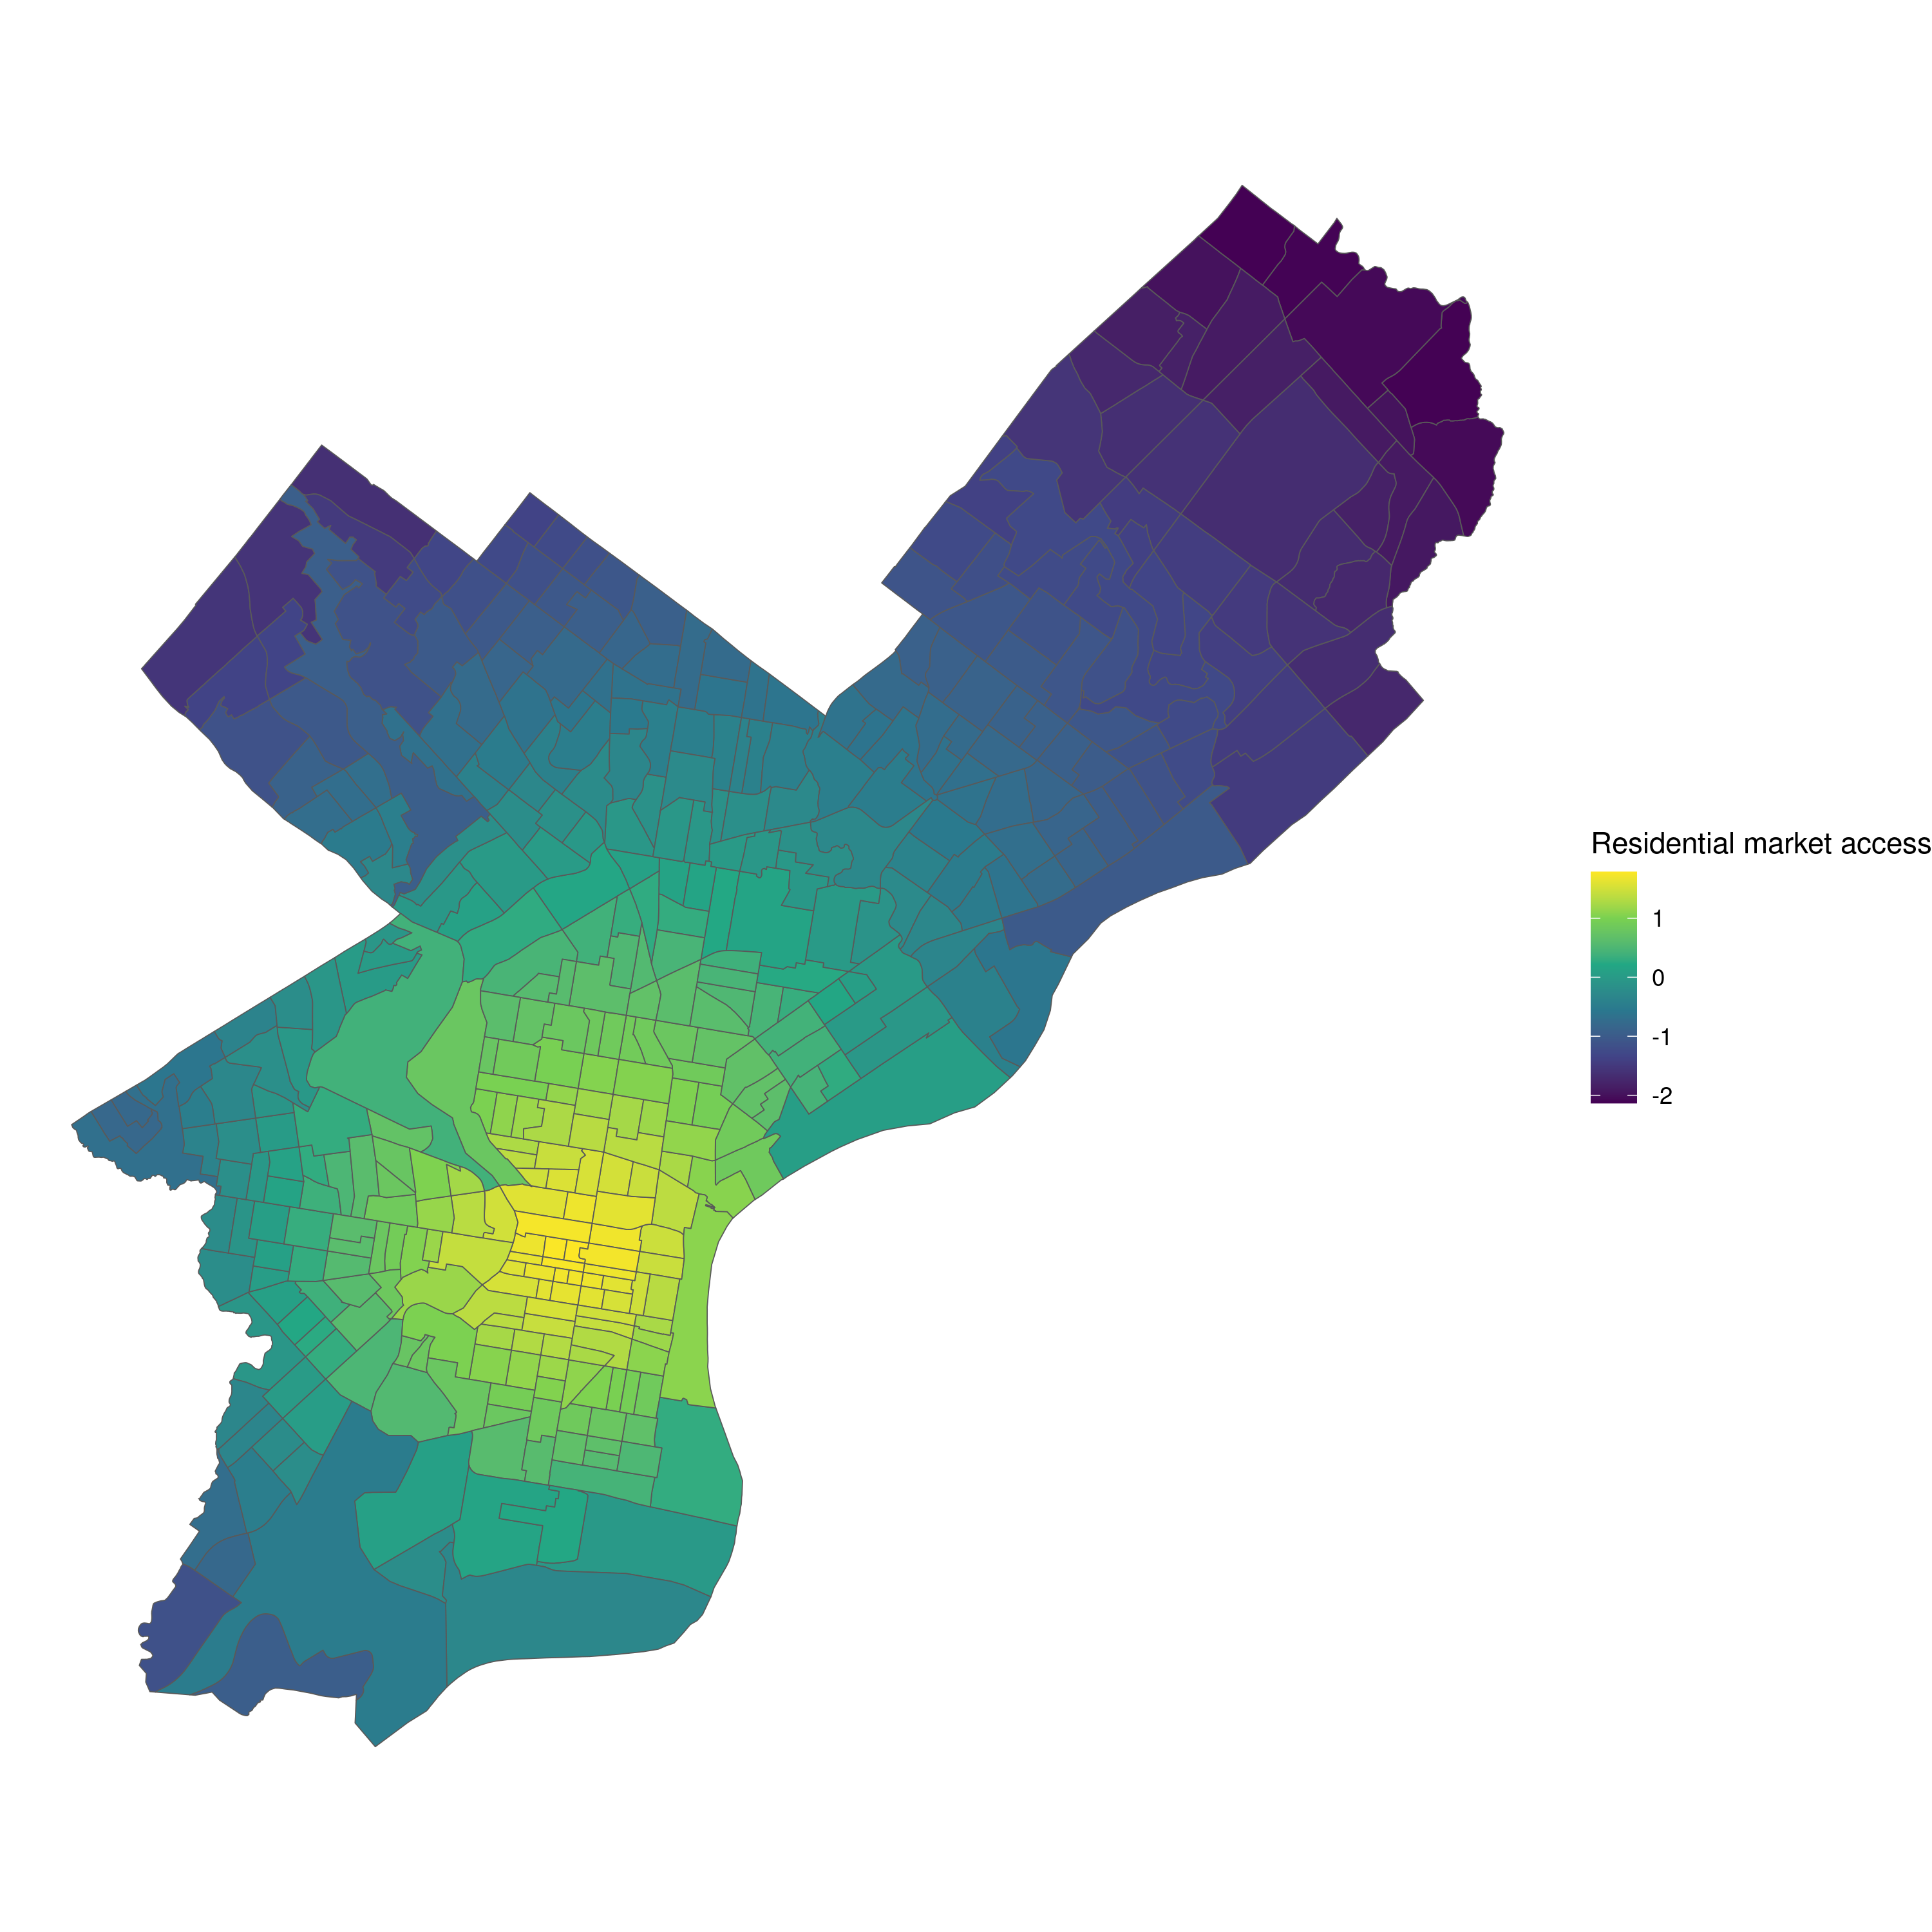
\includegraphics[keepaspectratio]{figures/residential_market_access_fixed_point.png}}

}

\subcaption{\label{fig-residential-market-access-fixed-point}Map of the
residential market access}

\end{minipage}%
%
\begin{minipage}{0.50\linewidth}

\centering{

\pandocbounded{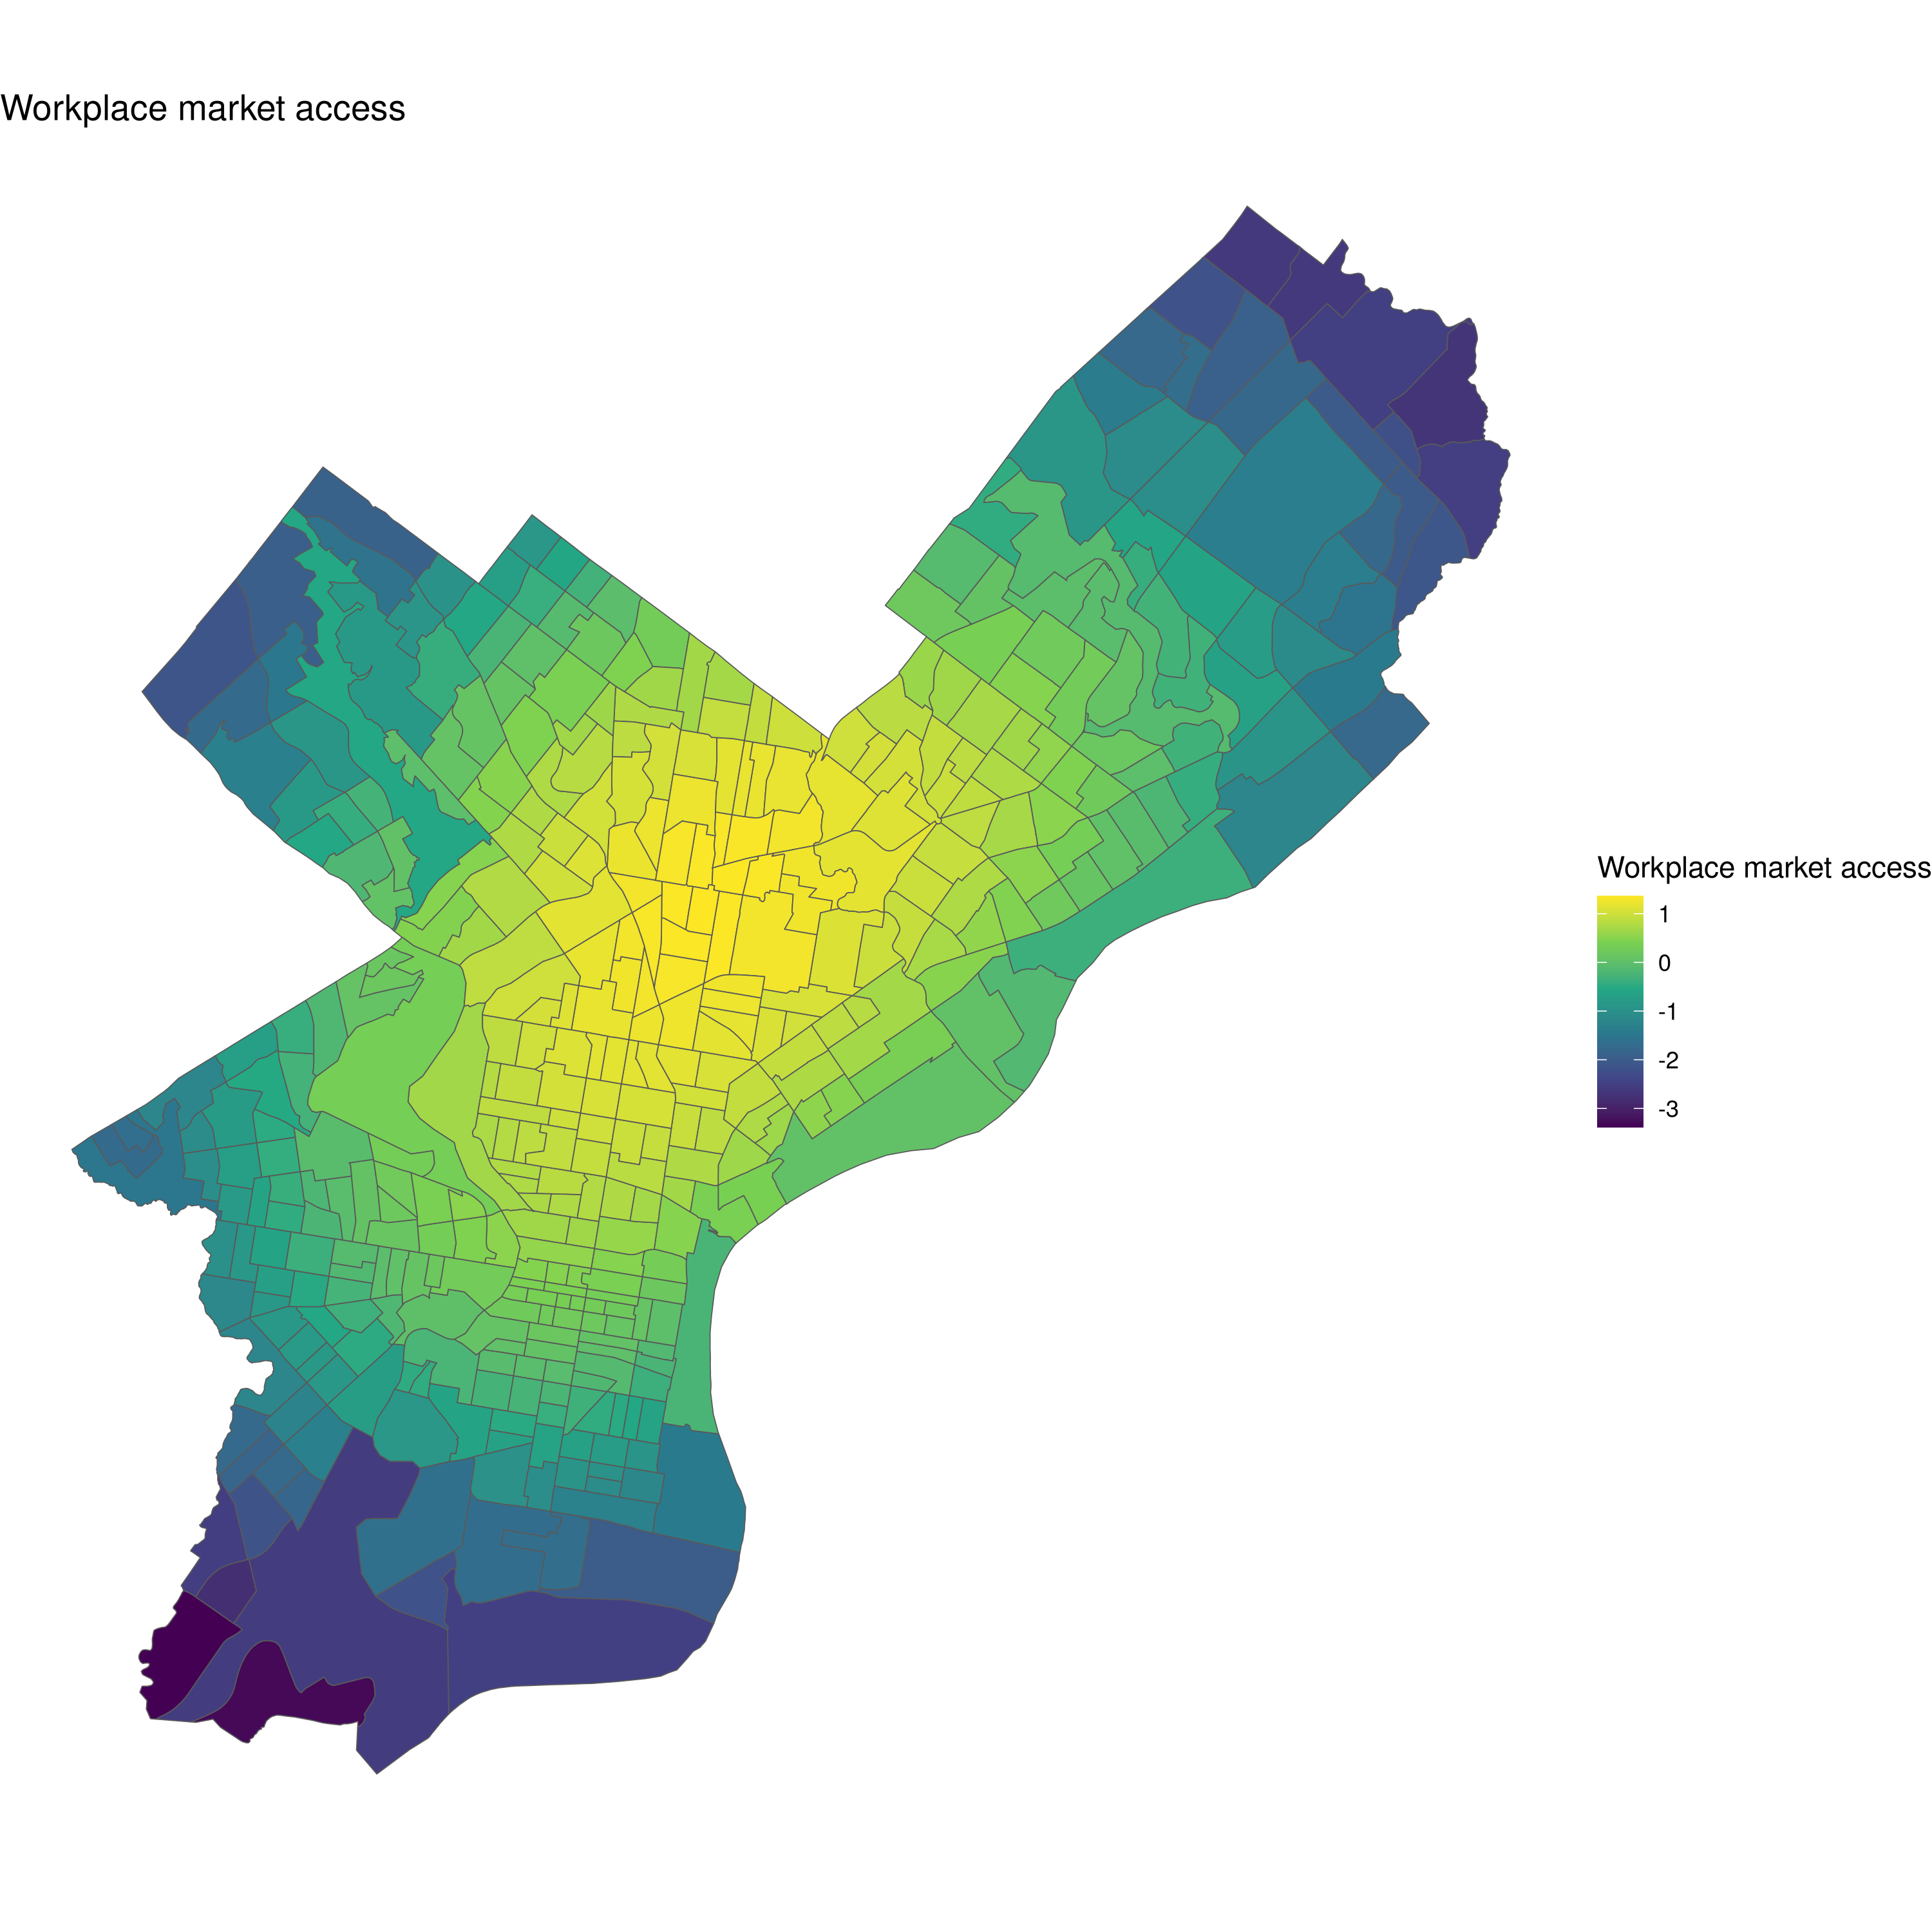
\includegraphics[keepaspectratio]{figures/workplace_market_access_fixed_point.png}}

}

\subcaption{\label{fig-workplace-market-access-fixed-point}Map of the
workplace market access}

\end{minipage}%

\end{figure}%

\footnotesize \textbf{Note}: This is the map (Philadelphia county) of
the market access variable. The color represents the market access
variable. The lighter the color, the higher the market access. The
values are normalized (z-score).

\normalsize

\section*{Q9}\label{q9}
\addcontentsline{toc}{section}{Q9}

While the level of the market access variable differs, the overall
distribution of the market access variable is similar. That is, the
ordinality of the market access variable is preserved for both cases.
This result is consistent with the derivation of the market access
equation we learned in class. To be specific, we discussed in page 21 of
the week1-lecture 1 that the equations in Q8 and Q9 are equivalent way
to derive market access variable. While the level of the market access
variable could differ, the ordinality of the market access variable
should be similar.

\section*{Q10}\label{q10}
\addcontentsline{toc}{section}{Q10}

Following Apppendix F of \citet{brinkman2024}, I need to create a fixed
point algorithm to solve for the following equation\footnote{I tweaked
  the equation from the paper to make it more clear for the matrix
  muliplication process I will be using below.}. (We will assume that
there are total \(J\) workplace tracts and \(I\) residential tracts.
While the number of tracts is same, we just use separate indices for
them to make it more clear in the equation.):

\begin{align*}
  \omega_j = \left( \frac{1}{N_{Wj}} \left[\sum_i \left( N_{Ri} \cdot d_{ij}^{-\epsilon}\right) \left[\sum_{j'} \left( w_{j'}^\epsilon \cdot d_{ij'}^{-\epsilon} \right)\right]^{-1}\right] \right)^{-\frac{1}{\epsilon}}
\end{align*}

I use the following matrix multiplication to setup the fixed point
algorithm (\(\omega = T(\omega)\)):

\begin{align*}
  \underbrace{
  \begin{bmatrix}
    \omega_1 \\
    \omega_2 \\
    \vdots \\
    \omega_J
  \end{bmatrix}}_{J \times 1}
  = &
  \overbrace{
  \begin{bmatrix}
    \left(\frac{1}{N_{W1}} \cdot N_{R1} \cdot d_{11}^{-\epsilon}\right) & \left(\frac{1}{N_{W1}} \cdot N_{R2} \cdot d_{21}^{-\epsilon}\right) & \ldots & \left(\frac{1}{N_{W1}} \cdot N_{RJ} \cdot d_{J1}^{-\epsilon}\right) \\
    \left(\frac{1}{N_{W2}} \cdot N_{R1} \cdot d_{12}^{-\epsilon}\right) & \left(\frac{1}{N_{W2}} \cdot N_{R2} \cdot d_{22}^{-\epsilon}\right) & \ldots \\
    \vdots & \vdots & \ddots \\
    \left(\frac{1}{N_{WJ}} \cdot N_{R1} \cdot d_{1J}^{-\epsilon}\right) & \left(\frac{1}{N_{WJ}} \cdot N_{R2} \cdot d_{2J}^{-\epsilon}\right) & \ldots & \left(\frac{1}{N_{WJ}} \cdot N_{RJ} \cdot d_{JJ}^{-\epsilon}\right) \\
  \end{bmatrix}}^{J \times I} \times \\ 
  &\underbrace{
  \begin{bmatrix}
    d_{11}^{-\epsilon} & d_{12}^{-\epsilon} & \ldots & d_{1J}^{-\epsilon} \\
    d_{21}^{-\epsilon} & d_{22}^{-\epsilon} & \ldots & d_{2J}^{-\epsilon} \\
    \vdots & \vdots & \ddots \\
    d_{I1}^{-\epsilon} & d_{I2}^{-\epsilon} & \ldots & d_{IJ}^{-\epsilon} \\
  \end{bmatrix}}_{I \times J} \times 
  \underbrace{
  \left(\begin{bmatrix}
    \omega_1 \\
    \omega_2 \\
    \vdots \\
    \omega_J
  \end{bmatrix}\right)^{\epsilon}}_{J \times 1}
\end{align*}

For convenience, I did not put the power of the \(-\frac{1}{\epsilon}\)
in the equation above. Also note that I also did not inverse the rows of
the matrix after the multiplication of \(I \times J\) and
\(J \times 1\). I will add them in the fixed point algorithm.

After retrieving the wages for each location, the rest is pretty
straightforward. This is because we no longer have the iterative
equations. We can just solve for the land rents, neighborhood amenities
and productivities using the equations in the Appendix F of
\citet{brinkman2024}.

I plot the map of the land rents in the following figure (Note that I
z-scored land rents and then used \texttt{asinh} transformation to make
the map more readable. This is because the land rents are very skewed
for certain tracts so raw values for other tracts become
indistinguishable in the map):

\clearpage

\begin{figure}

\centering{

\pandocbounded{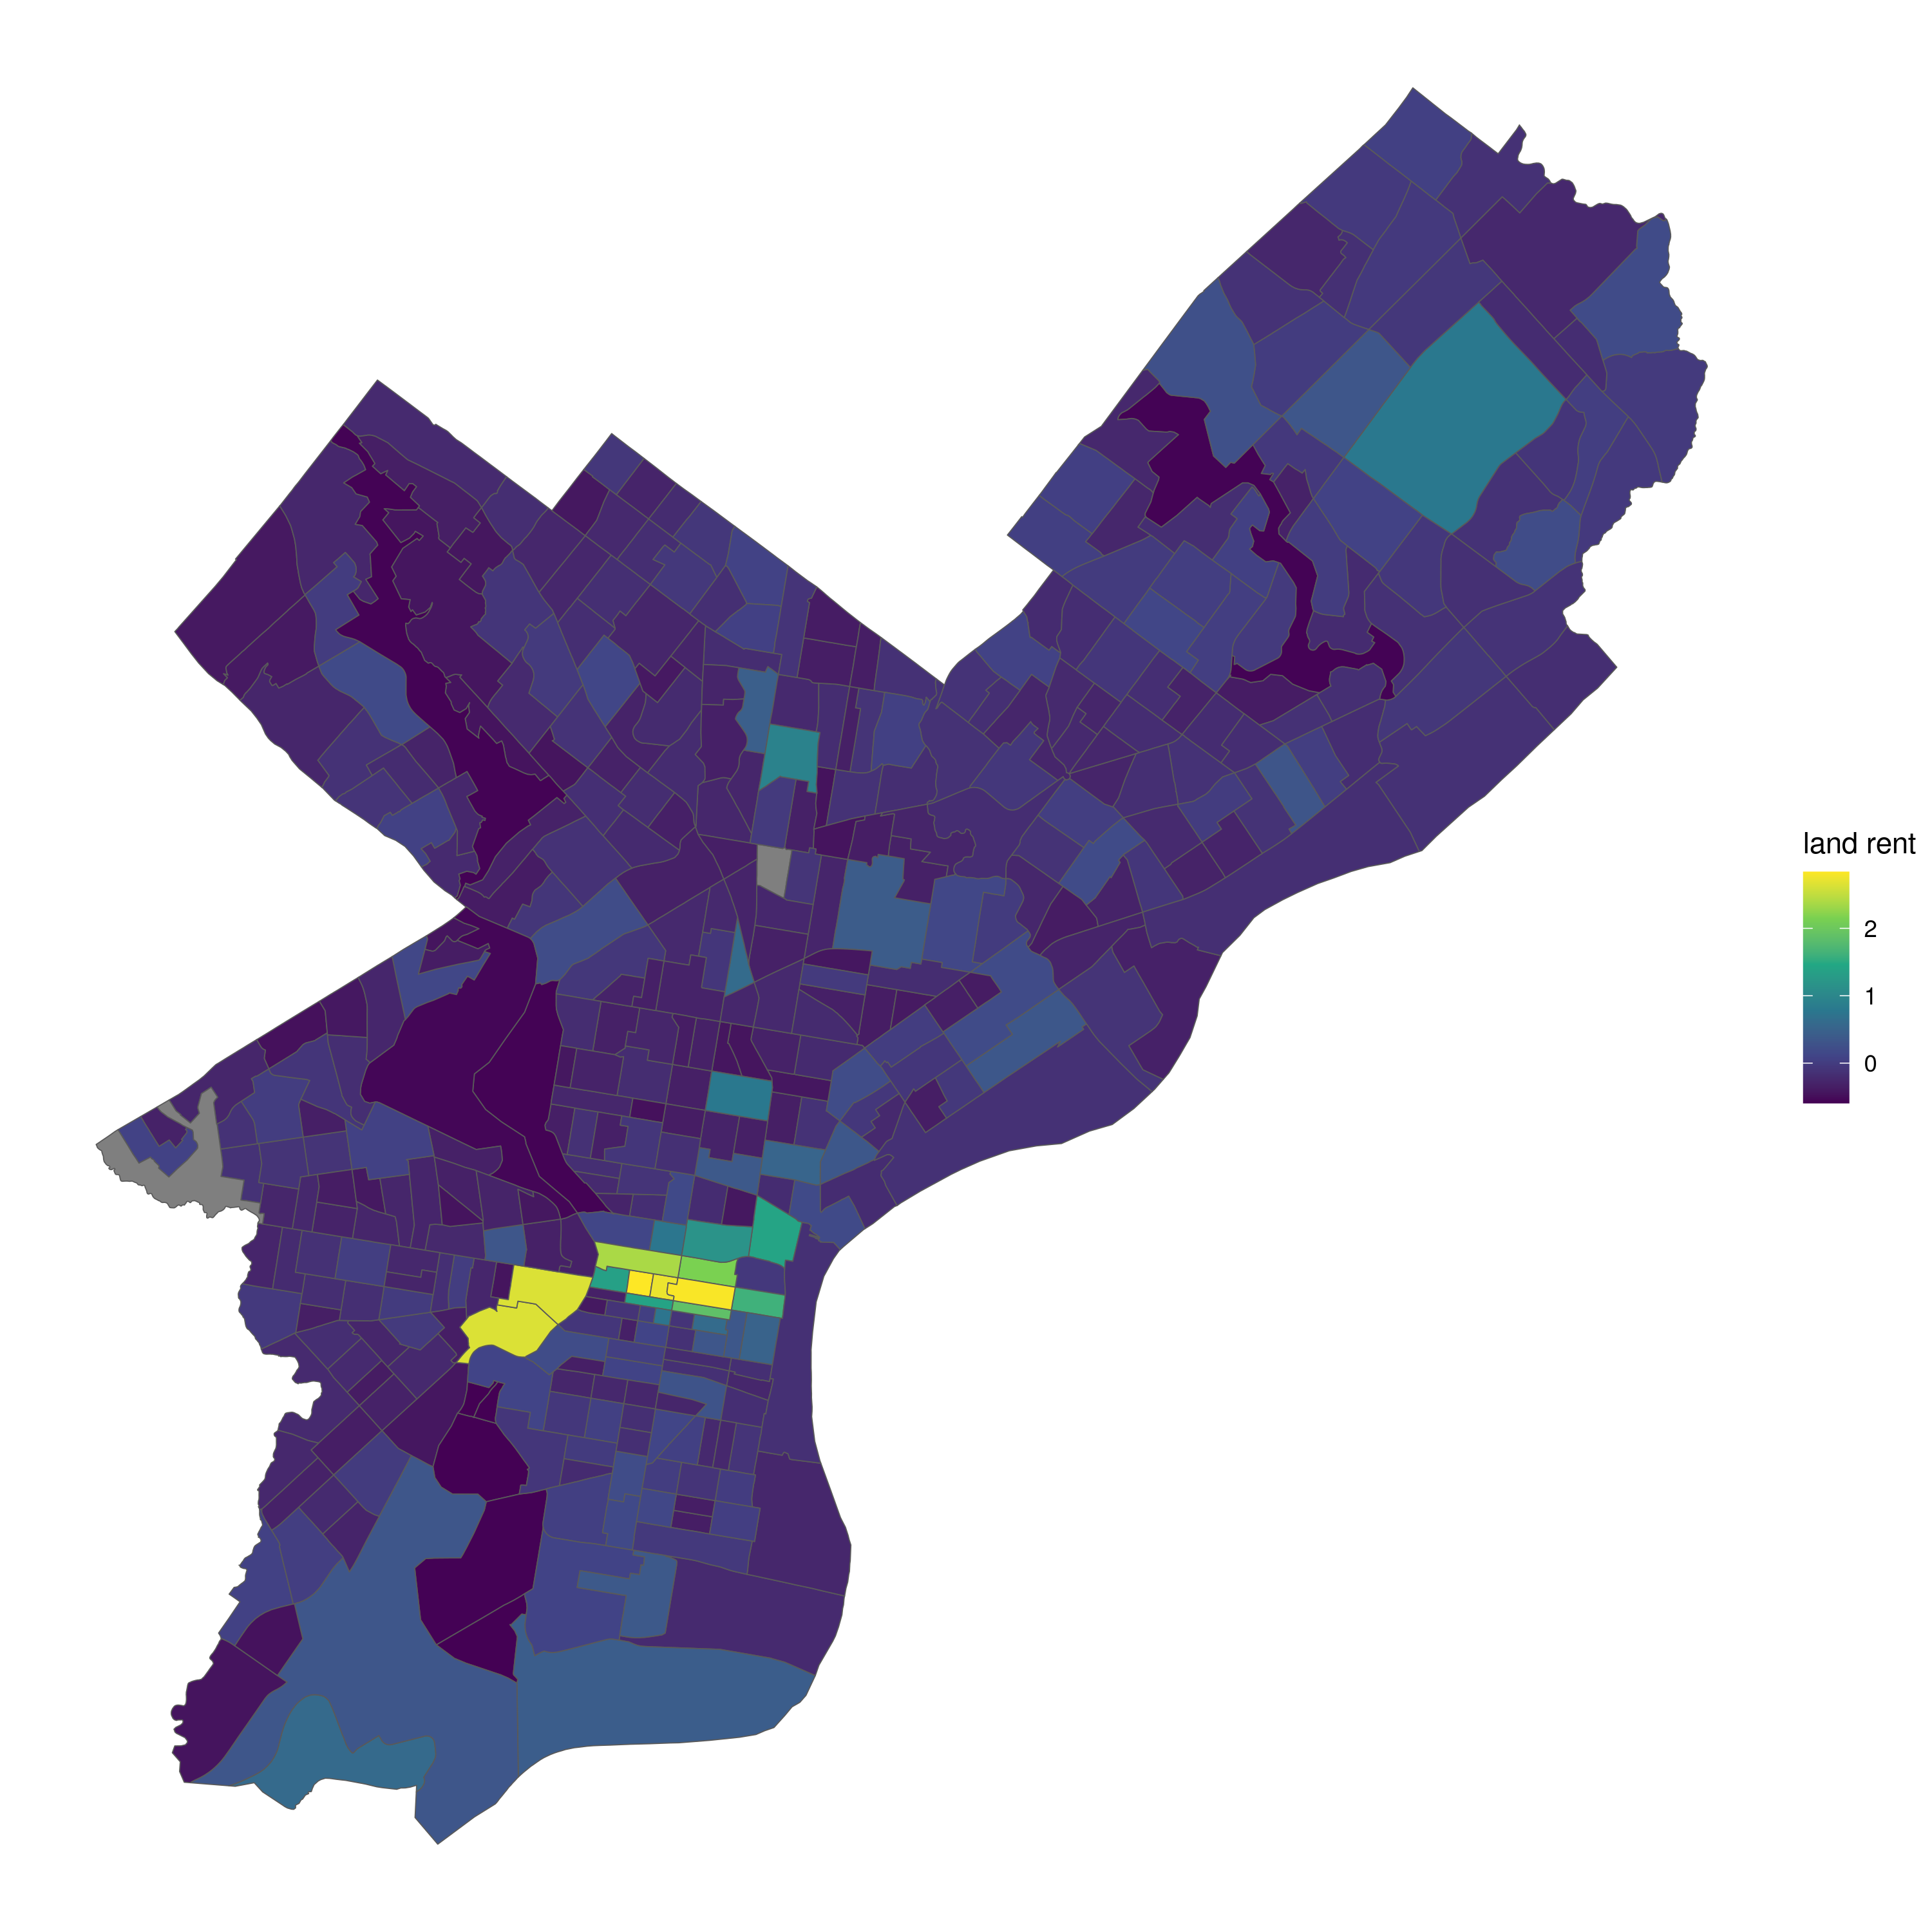
\includegraphics[keepaspectratio]{figures/land_rent.png}}

}

\caption{\label{fig-land-rent}Map of the land rents}

\end{figure}%

\footnotesize \textbf{Note}: This is the map (Philadelphia county) of
the land rents. The color represents the land rents. The lighter the
color, the higher the land rents. The values are normalized (z-score)
and then transformed using \texttt{asinh} transformation to make the map
more readable. The grey areas are tracts which we cannot recover the
land rents as there is no flow for them.\vspace{2em}

\normalsize

It is hard to say whether the land rents are reasonable or not but my
thoughts are that the results are not doing a good job of accurately
recovering the actual land rents. While the results seem to correctly
hint that regions near the center of the city have higher land rents,
this is also not very accurate as tracts that are more close to the
center of the city have lower land rents. According to some anecdotal
evidence, the land rents of the center of the city should be the highest
and the southern part of Philadelphia also should have relatively higher
land rents. These anecdotal evidence do not seem to be well captured by
the results.

I am assuming that this is because of the simplifying assumptions we
made. For example, we assumed that the land area is the same for all
tracts. This is of course not the accurate depiction of the actual land
areas of the tracts in Philadelphia county. Thus, these simplifying
assumptions might be leading to a more less accurate results.

\clearpage

\subsection*{References}\label{references}
\addcontentsline{toc}{subsection}{References}

\renewcommand{\bibsection}{}
\bibliography{bibliography.bib}

\clearpage

\phantomsection\label{appendix}
\bigskip

\begin{center}

{\large\bf APPENDIX}

\end{center}

\subsubsection*{A. Residential market
access}\label{a.-residential-market-access}
\addcontentsline{toc}{subsubsection}{A. Residential market access}


\begin{longtable}[t]{lr}
\caption{Residential market access}\\
\toprule
Tract & Residential market access\\
\midrule
\endfirsthead
\caption[]{Residential market access \textit{(continued)}}\\
\toprule
Tract & Residential market access\\
\midrule
\endhead

\endfoot
\bottomrule
\endlastfoot
42101000101 & 639.0000\\
42101000102 & 640.6758\\
42101000200 & 673.4206\\
42101000300 & 678.2559\\
42101000401 & 670.2414\\
42101000403 & 685.1711\\
42101000404 & 682.6896\\
42101000500 & 676.5047\\
42101000600 & 671.7848\\
42101000701 & 680.6982\\
42101000702 & 666.4638\\
42101000801 & 657.4542\\
42101000803 & 669.3243\\
42101000805 & 674.9733\\
42101000806 & 675.2463\\
42101000901 & 671.9652\\
42101000902 & 661.2686\\
42101001001 & 642.8700\\
42101001002 & 624.5171\\
42101001101 & 660.9236\\
42101001102 & 650.1898\\
42101001201 & 650.5192\\
42101001203 & 661.9271\\
42101001204 & 664.6579\\
42101001301 & 625.0713\\
42101001302 & 627.2692\\
42101001400 & 650.4874\\
42101001500 & 643.5468\\
42101001600 & 612.0793\\
42101001700 & 601.8734\\
42101001800 & 634.7687\\
42101001900 & 636.9506\\
42101002000 & 609.6598\\
42101002100 & 618.6535\\
42101002200 & 620.8187\\
42101002300 & 612.3581\\
42101002400 & 619.1416\\
42101002500 & 589.4441\\
42101002701 & 569.4423\\
42101002702 & 559.0235\\
42101002801 & 576.3334\\
42101002802 & 580.5149\\
42101002900 & 592.5586\\
42101003001 & 583.5872\\
42101003002 & 602.1961\\
42101003100 & 594.4223\\
42101003200 & 586.7031\\
42101003300 & 579.4188\\
42101003600 & 549.4329\\
42101003701 & 568.7620\\
42101003702 & 551.5565\\
42101003800 & 522.2531\\
42101003901 & 556.9414\\
42101003902 & 521.2855\\
42101004001 & 557.6791\\
42101004002 & 533.2719\\
42101004101 & 548.7410\\
42101004103 & 531.0104\\
42101004104 & 518.7471\\
42101004201 & 533.6831\\
42101004202 & 509.4160\\
42101005400 & 281.8948\\
42101005500 & 341.3808\\
42101005600 & 330.2170\\
42101006000 & 376.1246\\
42101006100 & 409.6979\\
42101006200 & 407.5095\\
42101006300 & 392.0841\\
42101006400 & 394.0980\\
42101006500 & 431.3316\\
42101006600 & 441.2349\\
42101006700 & 446.9330\\
42101007000 & 482.7128\\
42101007101 & 475.7183\\
42101007102 & 467.9034\\
42101007200 & 453.4342\\
42101007300 & 492.1773\\
42101007400 & 521.2860\\
42101007700 & 555.1971\\
42101007800 & 522.3426\\
42101007900 & 517.4734\\
42101008000 & 482.6838\\
42101008101 & 445.4927\\
42101008102 & 452.9123\\
42101008200 & 411.0564\\
42101008301 & 408.0891\\
42101008302 & 427.1449\\
42101008400 & 449.5292\\
42101008500 & 484.6198\\
42101008601 & 525.3391\\
42101008602 & 524.3084\\
42101008701 & 550.8184\\
42101008702 & 565.3760\\
42101008801 & 600.3704\\
42101008802 & 583.1702\\
42101009000 & 625.4096\\
42101009100 & 598.2004\\
42101009200 & 559.2041\\
42101009300 & 491.5433\\
42101009400 & 459.1726\\
42101009500 & 435.9880\\
42101009600 & 415.8959\\
42101009801 & 330.1410\\
42101009802 & 328.7922\\
42101010000 & 387.4578\\
42101010100 & 413.2522\\
42101010200 & 456.7518\\
42101010300 & 480.1786\\
42101010400 & 507.1256\\
42101010500 & 524.1736\\
42101010600 & 550.9300\\
42101010700 & 546.4358\\
42101010800 & 580.3830\\
42101010900 & 607.5471\\
42101011000 & 538.5288\\
42101011100 & 482.1394\\
42101011200 & 442.4112\\
42101011300 & 428.6951\\
42101011400 & 396.7748\\
42101011500 & 376.0446\\
42101011700 & 388.2408\\
42101011800 & 415.4358\\
42101011900 & 435.3099\\
42101012000 & 411.3600\\
42101012100 & 430.2246\\
42101012201 & 441.8152\\
42101012203 & 430.6568\\
42101012204 & 441.6685\\
42101012501 & 671.9002\\
42101012502 & 659.2144\\
42101013100 & 639.0221\\
42101013200 & 647.3801\\
42101013300 & 650.7982\\
42101013401 & 644.9685\\
42101013402 & 654.3969\\
42101013500 & 638.5013\\
42101013601 & 627.7545\\
42101013602 & 615.7008\\
42101013701 & 578.6255\\
42101013702 & 592.3935\\
42101013800 & 602.2377\\
42101013900 & 615.1503\\
42101014000 & 624.4697\\
42101014100 & 625.5866\\
42101014201 & 613.5777\\
42101014202 & 587.2259\\
42101014300 & 557.4811\\
42101014400 & 594.9821\\
42101014500 & 602.1715\\
42101014600 & 609.1908\\
42101014700 & 604.8572\\
42101014800 & 596.0196\\
42101014900 & 576.9084\\
42101015101 & 547.4438\\
42101015102 & 561.1559\\
42101015200 & 574.5095\\
42101015300 & 584.5237\\
42101015600 & 581.1293\\
42101015700 & 569.1920\\
42101015800 & 561.1395\\
42101016001 & 528.8269\\
42101016002 & 535.8077\\
42101016100 & 534.7923\\
42101016200 & 559.9389\\
42101016300 & 539.1046\\
42101016400 & 550.7822\\
42101016500 & 559.4170\\
42101016600 & 562.6348\\
42101016701 & 556.0416\\
42101016702 & 559.0593\\
42101016800 & 551.5746\\
42101016901 & 539.5065\\
42101016902 & 526.0103\\
42101017000 & 479.1791\\
42101017100 & 503.3389\\
42101017201 & 522.3727\\
42101017202 & 520.3500\\
42101017300 & 529.0001\\
42101017400 & 535.8038\\
42101017500 & 525.6673\\
42101017601 & 525.1571\\
42101017602 & 511.3244\\
42101017701 & 485.2691\\
42101017702 & 501.5694\\
42101017800 & 496.4707\\
42101017900 & 495.2146\\
42101018001 & 499.8963\\
42101018002 & 479.3902\\
42101018300 & 384.4940\\
42101018400 & 358.5857\\
42101018801 & 466.0756\\
42101018802 & 448.3871\\
42101019000 & 424.1777\\
42101019100 & 439.1390\\
42101019200 & 473.1725\\
42101019501 & 502.9275\\
42101019502 & 492.2711\\
42101019700 & 461.6481\\
42101019800 & 482.1233\\
42101019900 & 502.3473\\
42101020000 & 514.6614\\
42101020101 & 511.3105\\
42101020102 & 484.5948\\
42101020200 & 493.8577\\
42101020300 & 479.0565\\
42101020400 & 454.4671\\
42101020500 & 465.1930\\
42101020600 & 438.9276\\
42101020701 & 454.4426\\
42101020702 & 434.6432\\
42101020800 & 415.9339\\
42101020900 & 399.1675\\
42101021000 & 370.6438\\
42101021100 & 379.5433\\
42101021200 & 344.6698\\
42101021300 & 342.4444\\
42101021400 & 341.7439\\
42101021500 & 316.4123\\
42101021600 & 283.8316\\
42101021700 & 298.8882\\
42101021800 & 255.9215\\
42101021900 & 253.3480\\
42101022000 & 226.9578\\
42101023100 & 270.0637\\
42101023500 & 348.9650\\
42101023600 & 347.0276\\
42101023700 & 335.5456\\
42101023800 & 372.5118\\
42101023900 & 383.3058\\
42101024000 & 411.5514\\
42101024100 & 397.6487\\
42101024200 & 418.4115\\
42101024300 & 441.0418\\
42101024400 & 434.3326\\
42101024500 & 406.6449\\
42101024600 & 383.2250\\
42101024700 & 377.4058\\
42101024800 & 359.0840\\
42101024900 & 348.4772\\
42101025200 & 352.1052\\
42101025300 & 324.5738\\
42101025400 & 310.1485\\
42101025500 & 297.8573\\
42101025600 & 280.5762\\
42101025700 & 260.1727\\
42101025800 & 266.4706\\
42101025900 & 253.9764\\
42101026000 & 267.7110\\
42101026100 & 280.6895\\
42101026200 & 295.8520\\
42101026301 & 279.6965\\
42101026302 & 294.1406\\
42101026400 & 311.2792\\
42101026500 & 325.8418\\
42101026600 & 312.5227\\
42101026700 & 340.0431\\
42101026800 & 337.9593\\
42101026900 & 336.9184\\
42101027000 & 356.5222\\
42101027100 & 352.5953\\
42101027200 & 356.4233\\
42101027300 & 381.6673\\
42101027401 & 387.9924\\
42101027402 & 384.6153\\
42101027500 & 385.3481\\
42101027600 & 378.2633\\
42101027700 & 353.1487\\
42101027800 & 380.4554\\
42101027901 & 367.6907\\
42101027902 & 395.7932\\
42101028000 & 433.0786\\
42101028100 & 419.4801\\
42101028200 & 404.8556\\
42101028300 & 433.1487\\
42101028400 & 433.8737\\
42101028500 & 420.1585\\
42101028600 & 416.1862\\
42101028700 & 438.8209\\
42101028800 & 432.0812\\
42101028901 & 435.3682\\
42101028902 & 418.0814\\
42101029000 & 402.3728\\
42101029100 & 379.1325\\
42101029200 & 399.8514\\
42101029300 & 404.0152\\
42101029400 & 397.5810\\
42101029800 & 355.4927\\
42101029900 & 371.6060\\
42101030000 & 372.0573\\
42101030100 & 387.2301\\
42101030200 & 368.6597\\
42101030501 & 355.6924\\
42101030502 & 352.6397\\
42101030600 & 333.9988\\
42101030700 & 314.7596\\
42101030800 & 315.8147\\
42101030900 & 340.7243\\
42101031000 & 319.5549\\
42101031101 & 336.7175\\
42101031102 & 351.3562\\
42101031200 & 346.3529\\
42101031300 & 331.4838\\
42101031401 & 318.2673\\
42101031402 & 314.3150\\
42101031501 & 304.9002\\
42101031502 & 312.2304\\
42101031600 & 325.0097\\
42101031700 & 341.0305\\
42101031800 & 352.8577\\
42101031900 & 343.6274\\
42101032000 & 323.1147\\
42101032100 & 337.5216\\
42101032300 & 321.2726\\
42101032500 & 307.4262\\
42101032600 & 295.8897\\
42101032900 & 269.9287\\
42101033000 & 284.2097\\
42101033101 & 286.4497\\
42101033102 & 267.1389\\
42101033200 & 293.5419\\
42101033300 & 281.2045\\
42101033400 & 292.9157\\
42101033500 & 302.9882\\
42101033600 & 286.6009\\
42101033701 & 268.8173\\
42101033702 & 269.4683\\
42101033800 & 294.5977\\
42101033900 & 288.9652\\
42101034000 & 277.0992\\
42101034100 & 268.7952\\
42101034200 & 249.1374\\
42101034400 & 225.7288\\
42101034501 & 250.5875\\
42101034502 & 240.7516\\
42101034600 & 241.9969\\
42101034701 & 257.4649\\
42101034702 & 259.7915\\
42101034801 & 245.2731\\
42101034802 & 236.7287\\
42101034803 & 223.5891\\
42101034900 & 239.8300\\
42101035100 & 201.6585\\
42101035200 & 210.6546\\
42101035301 & 202.7452\\
42101035302 & 209.0877\\
42101035500 & 220.8810\\
42101035601 & 215.8845\\
42101035602 & 201.8845\\
42101035701 & 190.3363\\
42101035702 & 186.2169\\
42101035800 & 167.6235\\
42101035900 & 180.3865\\
42101036000 & 188.4499\\
42101036100 & 178.1919\\
42101036201 & 189.3246\\
42101036202 & 178.3022\\
42101036203 & 176.5044\\
42101036301 & 157.7371\\
42101036302 & 168.9168\\
42101036303 & 149.4473\\
42101036400 & 157.2073\\
42101036501 & 148.7052\\
42101036502 & 150.4102\\
42101036600 & 589.9003\\
42101036700 & 627.5988\\
42101036901 & 600.3949\\
42101036902 & 634.8801\\
42101037200 & 500.0666\\
42101037300 & 461.2565\\
42101037500 & 359.0122\\
42101037600 & 662.1399\\
42101037700 & 584.2287\\
42101037800 & 447.5264\\
42101037900 & 433.6444\\
42101038000 & 392.2234\\
42101038100 & 300.6101\\
42101038200 & 439.9720\\
42101038301 & 471.2053\\
42101038400 & 224.6463\\
42101038500 & 235.5893\\
42101038600 & 283.8498\\
42101038700 & 217.8781\\
42101038800 & 300.2375\\
42101038900 & 334.0411\\
42101039001 & 356.3713\\
42101039002 & 374.6660\\
42101039100 & 507.4218\\
42101980001 & 549.0917\\
42101980002 & 495.2708\\
42101980003 & 646.2937\\
42101980100 & 311.2988\\
42101980200 & 266.3802\\
42101980300 & 210.8902\\
42101980400 & 309.6947\\
42101980500 & 460.6334\\
42101980600 & 468.7767\\
42101980701 & 436.8104\\
42101980702 & 481.4650\\
42101980800 & 347.2216\\
42101980901 & 372.1682\\
42101980902 & 545.8168\\
42101980903 & 552.1639\\
42101980904 & 514.6799\\
42101980905 & 411.5504\\
42101980906 & 453.9761\\
42101989100 & 237.4495\\
42101989200 & 396.5034\\
42101989300 & 462.7540\\*
\end{longtable}


\clearpage

\subsubsection*{B.Workplace market
access}\label{b.workplace-market-access}
\addcontentsline{toc}{subsubsection}{B.Workplace market access}


\begin{longtable}[t]{lr}
\caption{Workplace market access}\\
\toprule
Tract & Workplace market access\\
\midrule
\endfirsthead
\caption[]{Workplace market access \textit{(continued)}}\\
\toprule
Tract & Workplace market access\\
\midrule
\endhead

\endfoot
\bottomrule
\endlastfoot
42101000101 & 331.4840\\
42101000102 & 337.9878\\
42101000200 & 345.4749\\
42101000300 & 349.9454\\
42101000401 & 345.1504\\
42101000403 & 344.8803\\
42101000404 & 345.6363\\
42101000500 & 341.1504\\
42101000600 & 337.4256\\
42101000701 & 341.9882\\
42101000702 & 341.8906\\
42101000801 & 338.6716\\
42101000803 & 339.6434\\
42101000805 & 339.2713\\
42101000806 & 338.4394\\
42101000901 & 336.7541\\
42101000902 & 333.0399\\
42101001001 & 327.1541\\
42101001002 & 321.7439\\
42101001101 & 332.2224\\
42101001102 & 328.2393\\
42101001201 & 334.5587\\
42101001203 & 335.3536\\
42101001204 & 334.6199\\
42101001301 & 323.6545\\
42101001302 & 326.3937\\
42101001400 & 330.1226\\
42101001500 & 325.4155\\
42101001600 & 314.4142\\
42101001700 & 309.6775\\
42101001800 & 321.9992\\
42101001900 & 325.0010\\
42101002000 & 317.7753\\
42101002100 & 318.9383\\
42101002200 & 318.0861\\
42101002300 & 313.3564\\
42101002400 & 315.8061\\
42101002500 & 303.7149\\
42101002701 & 294.2042\\
42101002702 & 289.4822\\
42101002801 & 297.3771\\
42101002802 & 299.4857\\
42101002900 & 305.3095\\
42101003001 & 302.3096\\
42101003002 & 310.5162\\
42101003100 & 308.7905\\
42101003200 & 307.6822\\
42101003300 & 310.1388\\
42101003600 & 291.8577\\
42101003701 & 297.3887\\
42101003702 & 289.0535\\
42101003800 & 273.2181\\
42101003901 & 289.5234\\
42101003902 & 270.5515\\
42101004001 & 288.8774\\
42101004002 & 276.1981\\
42101004101 & 283.9717\\
42101004103 & 274.6748\\
42101004104 & 267.9692\\
42101004201 & 276.4885\\
42101004202 & 263.3043\\
42101005400 & 155.0103\\
42101005500 & 196.3160\\
42101005600 & 183.9102\\
42101006000 & 215.5949\\
42101006100 & 232.2290\\
42101006200 & 236.1757\\
42101006300 & 231.2961\\
42101006400 & 236.0594\\
42101006500 & 262.5618\\
42101006600 & 259.2734\\
42101006700 & 256.0467\\
42101007000 & 280.2222\\
42101007101 & 281.2050\\
42101007102 & 281.4755\\
42101007200 & 279.7674\\
42101007300 & 294.0393\\
42101007400 & 298.1760\\
42101007700 & 312.8857\\
42101007800 & 304.9115\\
42101007900 & 307.9621\\
42101008000 & 296.9673\\
42101008101 & 280.1668\\
42101008102 & 287.0517\\
42101008200 & 264.8283\\
42101008301 & 270.9107\\
42101008302 & 279.5635\\
42101008400 & 290.8921\\
42101008500 & 303.7313\\
42101008601 & 313.5947\\
42101008602 & 316.5447\\
42101008701 & 320.0707\\
42101008702 & 323.7322\\
42101008801 & 331.3929\\
42101008802 & 326.6328\\
42101009000 & 343.4481\\
42101009100 & 337.5854\\
42101009200 & 329.2480\\
42101009300 & 311.0737\\
42101009400 & 299.5737\\
42101009500 & 291.5802\\
42101009600 & 281.5289\\
42101009801 & 239.7282\\
42101009802 & 237.0594\\
42101010000 & 270.6680\\
42101010100 & 285.5205\\
42101010200 & 302.5542\\
42101010300 & 311.6431\\
42101010400 & 319.2008\\
42101010500 & 325.7130\\
42101010600 & 331.7782\\
42101010700 & 334.8699\\
42101010800 & 341.4367\\
42101010900 & 347.2031\\
42101011000 & 337.5678\\
42101011100 & 318.4473\\
42101011200 & 300.6966\\
42101011300 & 298.0125\\
42101011400 & 282.9075\\
42101011500 & 268.6373\\
42101011700 & 285.4119\\
42101011800 & 296.1489\\
42101011900 & 306.9665\\
42101012000 & 302.1013\\
42101012100 & 313.3525\\
42101012201 & 331.3963\\
42101012203 & 329.4754\\
42101012204 & 326.0789\\
42101012501 & 354.0397\\
42101012502 & 354.1160\\
42101013100 & 355.5792\\
42101013200 & 359.2129\\
42101013300 & 360.5662\\
42101013401 & 357.8656\\
42101013402 & 359.0146\\
42101013500 & 362.4577\\
42101013601 & 358.7500\\
42101013602 & 359.8413\\
42101013701 & 358.2420\\
42101013702 & 361.2490\\
42101013800 & 364.4154\\
42101013900 & 366.3388\\
42101014000 & 366.9819\\
42101014100 & 363.1066\\
42101014201 & 354.9380\\
42101014202 & 341.5456\\
42101014300 & 340.7437\\
42101014400 & 359.1818\\
42101014500 & 367.4527\\
42101014600 & 369.1783\\
42101014700 & 370.9318\\
42101014800 & 370.1999\\
42101014900 & 364.6529\\
42101015101 & 361.4167\\
42101015102 & 366.7811\\
42101015200 & 372.4741\\
42101015300 & 374.6169\\
42101015600 & 368.2278\\
42101015700 & 363.8911\\
42101015800 & 353.3261\\
42101016001 & 353.0612\\
42101016002 & 359.1246\\
42101016100 & 366.6388\\
42101016200 & 372.0346\\
42101016300 & 374.4820\\
42101016400 & 378.4494\\
42101016500 & 378.7585\\
42101016600 & 378.7310\\
42101016701 & 378.1931\\
42101016702 & 378.9346\\
42101016800 & 375.9816\\
42101016901 & 371.0309\\
42101016902 & 364.7118\\
42101017000 & 364.9689\\
42101017100 & 371.0575\\
42101017201 & 376.9267\\
42101017202 & 372.9059\\
42101017300 & 380.8428\\
42101017400 & 382.7480\\
42101017500 & 383.4446\\
42101017601 & 379.3065\\
42101017602 & 379.9662\\
42101017701 & 371.8784\\
42101017702 & 374.8398\\
42101017800 & 366.9544\\
42101017900 & 358.5741\\
42101018001 & 348.5587\\
42101018002 & 345.8733\\
42101018300 & 324.2402\\
42101018400 & 314.0260\\
42101018801 & 364.4756\\
42101018802 & 362.2345\\
42101019000 & 369.4511\\
42101019100 & 376.1776\\
42101019200 & 374.6200\\
42101019501 & 382.8406\\
42101019502 & 383.9882\\
42101019700 & 388.9657\\
42101019800 & 388.1308\\
42101019900 & 386.5832\\
42101020000 & 384.9752\\
42101020101 & 384.0579\\
42101020102 & 385.0270\\
42101020200 & 381.2127\\
42101020300 & 386.8284\\
42101020400 & 384.9256\\
42101020500 & 378.7562\\
42101020600 & 360.5432\\
42101020701 & 354.8854\\
42101020702 & 344.5594\\
42101020800 & 345.6461\\
42101020900 & 325.0762\\
42101021000 & 312.5291\\
42101021100 & 324.1490\\
42101021200 & 307.6727\\
42101021300 & 301.1041\\
42101021400 & 294.1455\\
42101021500 & 280.9498\\
42101021600 & 256.7518\\
42101021700 & 278.0622\\
42101021800 & 247.6980\\
42101021900 & 237.0822\\
42101022000 & 216.4008\\
42101023100 & 277.2647\\
42101023500 & 320.8515\\
42101023600 & 326.1234\\
42101023700 & 326.9854\\
42101023800 & 346.3838\\
42101023900 & 344.9926\\
42101024000 & 359.2402\\
42101024100 & 359.3447\\
42101024200 & 369.1474\\
42101024300 & 371.4863\\
42101024400 & 376.1160\\
42101024500 & 372.2174\\
42101024600 & 358.7281\\
42101024700 & 362.3034\\
42101024800 & 353.8966\\
42101024900 & 353.1951\\
42101025200 & 343.7685\\
42101025300 & 326.8749\\
42101025400 & 322.8253\\
42101025500 & 309.6599\\
42101025600 & 294.0849\\
42101025700 & 274.1429\\
42101025800 & 287.0953\\
42101025900 & 278.9825\\
42101026000 & 293.8889\\
42101026100 & 302.2309\\
42101026200 & 316.8977\\
42101026301 & 306.2551\\
42101026302 & 320.0560\\
42101026400 & 330.9716\\
42101026500 & 343.2765\\
42101026600 & 336.5560\\
42101026700 & 354.0159\\
42101026800 & 354.8655\\
42101026900 & 355.9496\\
42101027000 & 366.7929\\
42101027100 & 366.7421\\
42101027200 & 370.4162\\
42101027300 & 380.5072\\
42101027401 & 381.0140\\
42101027402 & 380.6708\\
42101027500 & 379.2567\\
42101027600 & 374.5117\\
42101027700 & 359.5898\\
42101027800 & 372.3572\\
42101027901 & 364.4596\\
42101027902 & 373.9277\\
42101028000 & 381.7070\\
42101028100 & 382.1614\\
42101028200 & 382.2993\\
42101028300 & 386.4100\\
42101028400 & 387.9287\\
42101028500 & 387.0439\\
42101028600 & 387.2033\\
42101028700 & 388.7653\\
42101028800 & 387.8926\\
42101028901 & 384.4037\\
42101028902 & 384.2889\\
42101029000 & 384.9835\\
42101029100 & 379.8245\\
42101029200 & 379.1768\\
42101029300 & 367.3678\\
42101029400 & 356.9589\\
42101029800 & 343.9695\\
42101029900 & 349.1712\\
42101030000 & 358.8020\\
42101030100 & 369.6727\\
42101030200 & 367.5814\\
42101030501 & 372.9068\\
42101030502 & 371.0925\\
42101030600 & 363.2370\\
42101030700 & 352.2753\\
42101030800 & 354.2040\\
42101030900 & 366.9182\\
42101031000 & 356.4141\\
42101031101 & 364.2985\\
42101031102 & 369.3121\\
42101031200 & 365.4537\\
42101031300 & 358.9515\\
42101031401 & 353.6790\\
42101031402 & 348.9031\\
42101031501 & 334.3933\\
42101031502 & 343.5167\\
42101031600 & 347.0483\\
42101031700 & 356.5637\\
42101031800 & 364.9495\\
42101031900 & 347.7157\\
42101032000 & 338.3672\\
42101032100 & 333.3205\\
42101032300 & 327.4681\\
42101032500 & 323.7276\\
42101032600 & 318.4613\\
42101032900 & 301.1715\\
42101033000 & 311.6156\\
42101033101 & 320.9282\\
42101033102 & 305.6180\\
42101033200 & 330.7407\\
42101033300 & 326.0310\\
42101033400 & 336.3907\\
42101033500 & 345.4308\\
42101033600 & 334.0574\\
42101033701 & 318.6734\\
42101033702 & 320.2811\\
42101033800 & 340.0937\\
42101033900 & 332.4779\\
42101034000 & 325.7448\\
42101034100 & 316.7976\\
42101034200 & 299.5119\\
42101034400 & 277.8562\\
42101034501 & 301.6243\\
42101034502 & 292.0612\\
42101034600 & 290.3197\\
42101034701 & 306.5584\\
42101034702 & 305.6629\\
42101034801 & 288.5876\\
42101034802 & 283.3962\\
42101034803 & 267.8079\\
42101034900 & 275.9948\\
42101035100 & 234.6829\\
42101035200 & 250.1116\\
42101035301 & 245.5095\\
42101035302 & 254.1949\\
42101035500 & 270.3945\\
42101035601 & 266.9312\\
42101035602 & 252.1731\\
42101035701 & 239.2081\\
42101035702 & 234.9803\\
42101035800 & 214.3758\\
42101035900 & 227.6205\\
42101036000 & 234.2275\\
42101036100 & 222.5089\\
42101036201 & 234.1495\\
42101036202 & 222.2368\\
42101036203 & 218.3934\\
42101036301 & 197.1701\\
42101036302 & 212.2746\\
42101036303 & 189.3769\\
42101036400 & 197.7548\\
42101036501 & 191.9882\\
42101036502 & 192.7524\\
42101036600 & 309.7801\\
42101036700 & 345.8318\\
42101036901 & 322.3850\\
42101036902 & 336.3060\\
42101037200 & 257.4414\\
42101037300 & 238.1645\\
42101037500 & 262.6108\\
42101037600 & 350.9743\\
42101037700 & 373.9169\\
42101037800 & 324.3067\\
42101037900 & 340.4407\\
42101038000 & 346.3047\\
42101038100 & 304.1158\\
42101038200 & 355.2406\\
42101038301 & 388.0286\\
42101038400 & 225.3713\\
42101038500 & 244.2117\\
42101038600 & 280.9694\\
42101038700 & 228.8420\\
42101038800 & 301.6565\\
42101038900 & 341.2597\\
42101039001 & 372.7660\\
42101039002 & 376.5146\\
42101039100 & 285.2360\\
42101980001 & 354.3594\\
42101980002 & 338.5074\\
42101980003 & 347.4473\\
42101980100 & 294.4942\\
42101980200 & 316.6515\\
42101980300 & 254.2309\\
42101980400 & 158.7578\\
42101980500 & 388.1144\\
42101980600 & 239.2324\\
42101980701 & 222.7676\\
42101980702 & 250.1787\\
42101980800 & 246.7172\\
42101980901 & 194.9220\\
42101980902 & 298.8449\\
42101980903 & 299.4402\\
42101980904 & 279.3537\\
42101980905 & 213.7029\\
42101980906 & 240.9222\\
42101989100 & 262.8361\\
42101989200 & 198.4836\\
42101989300 & 384.5268\\*
\end{longtable}






\end{document}
